\chapter{Flavors of oddness in non-scalar Hurford sentences}\label{chap:hurford-sentences}



	\textbf{Abstract. } A recent line of research (\cite{Katzir2015} i.a.) develops the idea that felicitous sentences should constitute possible answers to a ``good'' Question under Discussion (QuD, \cite{Roberts1996,VanKuppevelt1995}). In this chapter, we develop a compositional machinery formalizing the pairing process between assertions and implicit QuDs, and show that rephrasing two pragmatic principles (\textsc{Relevance}, \textsc{Redundancy}) in light of this new machinery  allows to solve puzzles pertaining to Hurford Disjunctions \cite{Hurford1974} and variants thereof \cite{Marty2022,Mandelkern2018}. More broadly, this motivates the use of QuDs as an explanatory tool for pragmatics.





\section{Introduction}

Hurford Disjunctions (henceforth, HD, \cite{Hurford1974}), exemplified in (\ref{ex:hd}), typically feature entailing disjuncts, and are generally odd regardless of the order of the weak ($p$) vs. strong ($p^+$) disjunct.\footnote{A notable exception is when the two disjuncts are the same modulo scalemate expressions, such as \textit{some} vs. \textit{all}; in that case, HDs may be rescued from infelicity (\cite{Gazdar1979,Singh2008b,Fox2018,HenotMortier2022} i.a.). We do not cover these cases here, but \cite{HenotMortier2024a} and Chapter 4 provides an overview of the challenges raised by ``scalar'' Hurford Disjunctions and Conditionals, and sketches a potential account of the latter building directly on the framework presented here.}

\begin{exe}
	\ex \label{ex:hd}
	\begin{xlist}
		\ex[\#] {SuB29 will take place in Noto\footnote{Noto is located in Italy and is where the main session of SuB29 was organized.} or Italy. \hfill $p^+\vee p$}\label{ex:hd-sw}
		\ex[\#] {SuB29 will take place in Italy or Noto. \hfill $p \vee p^+$}\label{ex:hd-ws}
	\end{xlist}
\end{exe}

\citet{Mandelkern2018} observed that Hurford Conditionals (henceforth HC), exemplified in (\ref{ex:hc}), can be directly derived from (\ref{ex:hd-sw}) \textit{via} the \textit{or-to-if} tautology and basic principles of classical logic (cf. \ref{ex:hd-hc-derivation}). Surprisingly, (\ref{ex:hc-sw}) and (\ref{ex:hc-ws}) exhibit a crisp oddness asymmetry. Descriptively, it seems that the weaker item has to appear in the antecedent of such conditionals, while the negated stronger item has to appear in the consequent.

\begin{exe}
	\ex \label{ex:hc}
	\begin{xlist}
		\ex[\#] {If SuB29 will not take place in Noto, it will take place in Italy. \hfill $\neg p^+\rightarrow p$}\label{ex:hc-sw}
		\ex[] {If SuB29 will take place in Italy, it will not take place in Noto. \hfill $p \rightarrow \neg p^+$}\label{ex:hc-ws}
	\end{xlist}
\end{exe}

\begin{exe}
	\ex \textit{Equivalence between HDs and HCs} \label{ex:hd-hc-derivation}
	\begin{xlist}
		\ex {(\ref{ex:hc-sw}) $\equiv \neg p^+\rightarrow p \stackrel{\clubsuit}{\equiv} \neg(\neg p^+)\vee p \stackrel{\spadesuit}{\equiv} p^+\vee p \equiv$ (\ref{ex:hd-sw})}
		\ex {(\ref{ex:hc-ws}) $\equiv p \rightarrow \neg p^+ \stackrel{\clubsuit}{\equiv} (\neg p) \vee (\neg p^+) \stackrel{\varheart}{\equiv} q^+\vee q \equiv$ (\ref{ex:hd-sw})\\
			$\clubsuit$: \textit{or-to-if} tautology; $\spadesuit$: double-negation elimination; $\varheart$: variable change of the form $\neg p := q^+; \neg p^+ := q$, with $q^+ \vDash q$.}
	\end{xlist}
\end{exe}
\citet{Kalomoiros2024} proposed the first solution to both (\ref{ex:hd}) and (\ref{ex:hc}), based on the idea that overt negation has a special status when it comes to evaluating if a sentence is redundant. In this chapter, I argue for an alternative view that builds on the general idea that felicitous assertions are ``good answers to good questions'' \cite{Katzir2015}. To operationalize this intuition in the context of Hurford Sentences, I use two core ingredients. The first is that declaratives evoke the potential QuDs they could answer, in the form of parse trees of the Context Set (in the spirit of \cite{Buring2003,Zhang2024}). Such QuD-trees ``match'' the degree of granularity of the assertion, and are compositionally derived; in particular, I submit that logically equivalent disjunctions and conditionals evoke \textit{distinct} kinds of trees. Roughly, disjunctions evoke QuD-trees making both disjuncts at issue \textit{at the same time}, while conditionals evoke QuD-trees linked to their consequent, but \textit{restricted} to the domains where their antecedent holds (a kind of neglect-zero effect, \cite{Aloni2022}). The second ingredient, is that some sentence-QuD pairings are ruled out due to violations of specific \textsc{Redundancy} and \textsc{Relevance} constraints. Roughly, a QuD-tree is redundant given a sentence if it is also evoked by a formal simplification of the sentence. A QuD-tree is irrelevant given a sentence, if at some point of its computation, its maximal true answers get altered (``cut-out''). This predicts the HDs in (\ref{ex:hd}) to be redundant, due to them evoking questions that are also evoked by their stronger disjunct. And this predicts the HC in (\ref{ex:hc-sw}) to be irrelevant, due to the fact that \textit{France}-worlds cannot properly ``fit'' within a \textit{not Paris} domain of the Context Set. The HC in (\ref{ex:hc-ws}) on the other hand, is correctly ruled-in due to the fact that \textit{not Paris}-worlds can be subdivided into a city partition, which properly fits within a \textit{France} domain of the Context Set.

The rest of this chapter is structured as follows. Section \ref{sec:prev-approaches} sketches two previous approaches to Hurford Sentences that are relevant to the current discussion, and outlines their limitations. Section \ref{sec:machinery} introduces the compositional machinery used to derive potential QuDs out of assertions. Section \ref{sec:constraints} defines two constraints (\textsc{Redundancy}, \textsc{Relevance}) on LF-QuD pairs and shows how such constraints capture the Hurford Sentences in (\ref{ex:hd}) and (\ref{ex:hc}). Section \ref{sec:ccl} concludes by showing how the account may capture other kinds of Hurford Sentences, while outlining what the remaining issues and questions may be.
\section{Previous approaches}\label{sec:prev-approaches}
In this section I briefly present two existing \textsc{Redundancy}-based accounts of Hurford Sentences: \textsc{Local Redundancy Checking} and \textsc{Super-Redundancy}. I show how the first account falls short in explaining HCs. I then show how the second account captures the contrast between HDs and HCs, discuss its core assumptions and potential limitations.
\subsection{Local Redundancy Checking}
\citet{Katzir2014} propose that the semantic computation evaluates, at
certain nodes, whether the semantic composition principle that applies there is non-vacuous. This gives rise to the principle in (\ref{ex:local-redundancy-checking}).
\begin{exe}
	\ex {\textit{Local Redundancy Checking.} $S$ is deviant if $S$ contains $\gamma$ s.t. $\llbracket \gamma \rrbracket = \llbracket O(\alpha, \beta) \rrbracket \equiv_c \llbracket\zeta \rrbracket, \ \zeta \in \lbrace \alpha, \beta\rbrace$.}\label{ex:local-redundancy-checking}
\end{exe}
This predicts the HDs in (\ref{ex:hd}) to be deviant, because both are contextually equivalent to one of their disjuncts. But, assuming conditionals denote material implications, this also predicts \textit{both} HCs in (\ref{ex:hc}) to be deviant. In those constructions, the only candidate for $\gamma$  is the whole conditional, with arguments $\neg p^+$ and $p$. (\ref{ex:hc-sw}) is contextually equivalent to $p$, and thus equivalent to its consequent; (\ref{ex:hc-sw}) is contextually equivalent to $\neg p^+$, and thus equivalent to its consequent, as well. 
The issue persists if we adopt a non-material analysis of conditionals, because, in such cases, the whole conditional will never be contextually equivalent to its antecedent or consequent, regardless of what they denote. In other words, both HCs in (\ref{ex:hc}) would be predicted to be non-deviant.


\iffalse
\subsection{Logical Integrity}

\citet{Anvari2018} proposed a principle forcing the logical relation between a sentence and its non-weaker alternatives to be preserved once contextual information is considered.

\begin{exe}
	\ex {\textit{Logical Integrity.} Let $S$ be a sentence and $S'$ be one of its alternatives. $S$ is infelicitous in a context $c$ if $S$ does not logically entail $S'$, but $S$ contextually entails $S'$ in $c$.}
\end{exe}

This predicts the HDs in (\ref{ex:hd}) to be deviant, because both have their weak disjunct as alternative, do not logically entail it, but do so once the contextual information that Noto is in Italy is considered. But, assuming conditionals denote material implications, this also predicts \textit{both} HCs in (\ref{ex:hc}) to be deviant. (\ref{ex:hc-sw}) has its consequent ($p$) as alternative, does not logically entail it, but does so once the contextual information that Noto is in Italy is considered. (\ref{ex:hc-ws}) has its consequent ($\neg p^+$) as alternative, does not logically entail it, but does so once the contextual information that Noto is in Italy (and thus, that not being in Italy means not being in Noto) is considered. 
The issue persists if we adopt a non-material analysis of conditionals, because, in such cases, it is unclear if the conditional even logically entails one of its alternatives, end even so, no contrast would be predicted between the two HCs.

\subsection{Non-triviality}
Another line of work, building on local contexts \citep{Schlenker2009}, associates redundancy with triviality in the spirit of \citep{Stalnaker1999}: a sentence should not contain a part that is trivially true or false when evaluated against its local context \citep{Mayr2016}.
\begin{exe}
	\ex {\textit{Non-triviality.} A sentence $S$ cannot be used in a context $c$ if some part $\pi$ of $S$ is entailed or contradicted by the local context of $\pi$ in $c$.}\label{ex:non-triviality}
\end{exe}

Assuming disjunctive local contexts are symmetric, this predicts the HDs (\ref{ex:hd}) to both be deviant, because in both cases the strong disjunct ends up being trivially false when interpreted in the context of the negation of the weaker disjunct. But, assuming conditionals denote material implications, this also predicts \textit{both} HCs in (\ref{ex:hc}) to be deviant. Assuming asymmetric (left-to-right) local contexts for conditionals does not help capturing the contrast either: in (\ref{ex:hc-sw}), the consequent $p$, is informative in the context created by the antecedent ($\neg p^+$): not being in Noto neither entails nor contradicts being in Italy. In (\ref{ex:hc-sw}), the consequent $\neg p^+$, is also informative in the context created by the antecedent ($p$): being in Italy neither entails nor contradicts not being in Noto. 

\fi

\subsection{Super-Redundancy}
%HDs feel redundant; while HCs sound locally irrelevant.
%Talk about repairs: the fact the repairs are differnt suggets the violation stems from a different source.
\citet{Kalomoiros2024} proposes an adaptation of (\ref{ex:local-redundancy-checking}), dubbed \textsc{Super-Redundancy}, which captures both (\ref{ex:hd}) and (\ref{ex:hc}). Roughly, a sentence is super-redundant if there is no way of strengthening one of its subconstituents that would make the resulting sentence non-redundant.


\begin{exe}
	\ex {\textit{Super-redundancy.} A sentence $S$ is infelicitous if it contains a subconstituent $C$ combining with a binary operator, s.t. $(S)^-_C$ is defined and for all $D$, $(S)^-_C \equiv S_{Str(C, D)}$.}
\end{exe}
$(S)^-_C$ in the above definition designates $S$ where $C$ got deleted, while $Str(C, D)$ refers to a strengthening of $C$ with $D$, defined inductively and whose key property is that it commutes with negation ($Str(\neg\alpha, D) = \neg (Str(\alpha, D))$), as well as with binary operators ($Str(O(\alpha, \beta), D) = O(Str(\alpha, D), Str(\beta, D))$). $S_{Str(C, D)}$ designates $S$ where $C$ is replaced by the strengthening of $C$ with $D$, $Str(C, D)$.\\

This predicts the HDs in (\ref{ex:hd}) to be deviant, because, given $C=p^+$, no matter what $D$ is, $S_{Str(C, D)} = (p^+\wedge D) \vee p$ is equivalent to $p=(S)^-_C$. This predicts the HC (\ref{ex:hc-sw}) to be deviant as well: given $C=\neg p^+$, no matter what $D$ is, $S_{Str(C, D)} = \neg(p^+\wedge D) \rightarrow p = (p^+ \wedge D) \vee p$ is equivalent to $p=(S)^-_C$. In that case, it was crucial that the local strengthening of $C=p^+$ remained conjunctive under negation. 
(\ref{ex:hc-ws}) on the other hand, is predicted to be fine: given $C=\neg p^+$, and setting $D$ to $\top$ we have, $S_{Str(C, D)} = p \rightarrow \neg(p^+\wedge \top) \equiv \neg p \vee \neg p^+$ which is \textit{not} equivalent to $p=(S)^-_C$. Given $C=p$, and setting $D$ to $\bot$ we have, $S_{Str(C, D)} = (p \wedge \bot) \rightarrow \neg p^+ \equiv \neg p \vee \top \vee \neg p^+\equiv\top$ which is \textit{not} equivalent to $\neg p^+=(S)^-_C$. In both cases, it was again crucial that the local strengthening of $C=p^+$ was conjunctive under negation (and thus, disjunctive after applying De Morgan's law).
\citet{Kalomoiros2024} also shows that this account extends to strict (yet not variably strict) conditionals.\\

This approach is compelling regarding Hurford Sentences and allows to retain a classical interpretation of the logical connectives. However, while traditional views of \textsc{Redundancy} link it to pragmatic principles such as \textsc{Brevity} \citep{Grice1975}, it remains unclear, under the \textsc{Super-Redundancy} view, why the notion of local strengthening ($Str$) is defined the way it is, and why it should be so central in deriving redundancy. Also, the account was originally motivated by the observation that negated HDs, like (\ref{ex:hd-neg}), appear felicitous.

\begin{exe}
	\ex {John either doesn't smoke or he doesn't smoke Marlboros.}\label{ex:hd-neg}
\end{exe}

While we agree with the above judgment, we think something else might be at stake in (\ref{ex:hd-neg}), given that it is improved by focus (\ref{ex:hd-neg-focus}), but made worse by removing \textit{either} (\ref{ex:hd-neg-no-either}), or by swapping the disjuncts (\ref{ex:hd-neg-swap}). The last two cases can be repaired by adding \textit{at all} to the stronger disjunct.\footnote{The same patterns can be amplified if the two disjuncts are made more parallel (i.e., instead of having $V$ and $V+NP$, we have $V+NP$ and $V+NP^+$, with $\llbracket NP^+\rrbracket \subset \llbracket NP\rrbracket$). This is done in (\ref{ex:hd-neg-parallel}) whose variants (analog to (\ref{ex:hd-neg-focus}-\ref{ex:hd-neg-swap})) are given in (\ref{ex:hd-neg-parallel-variants}).
	\begin{exe}
		\ex[?] {John either doesn’t own a dog or he doesn't own a lab.}\label{ex:hd-neg-parallel}
		\ex \label{ex:hd-neg-parallel-variants}
		\begin{xlist}
			\ex {John doesn’t own a dog or doesn't own a LAB.}
			\ex {John doesn’t own a dog ${}^{??}$(at all) or doesn't own a lab.}
			\ex {John either doesn't own a lab or he doesn't own a dog ${}^{\#}$(at all).}
		\end{xlist}
\end{exe}}

\begin{exe}
	\ex \label{ex:hd-neg-variants}
	\begin{xlist}
		\ex {John doesn’t smoke or doesn't smoke MARLBOROS.}\label{ex:hd-neg-focus}
		\ex {John doesn’t smoke ${}^?$(at all) or doesn't smoke Marlboros.}\label{ex:hd-neg-no-either}
		\ex {John either doesn't smoke Marlboros or he doesn't smoke ${}^{\#}$(at all).}\label{ex:hd-neg-swap}
	\end{xlist}
\end{exe}



This suggests that some pragmatic mechanism is at play in the weaker disjunct and makes it contradict the stronger one. In particular, \textit{John does not smoke MARLBOROS} seems to imply John smokes cigarettes of a brand different from Marlboros, i.e. smokes. While this does not alone explain the complex pattern of repairs in (\ref{ex:hd-neg-variants}) and (\ref{ex:hd-neg-parallel-variants}), this appears more in line with an analysis of HDs which would not assign a special status to overt negation, but instead interacts with other pragmatic processes which themselves, are constrained by negation. Lastly, \cite{Kalomoiros2024}'s \textsc{Super-Redundancy} is challenged by other varieties of redundant sentences obtained from the structure $p\vee p \vee q$ \textit{via} the \textit{or-to-if} tautology (see \citenp{HenotMortier2024b} and Chapter 3).

\section{Linking assertions to questions}\label{sec:machinery}


Building on the model proposed for Hurford Sentences by \citet{HenotMortier2024} and previous work by \cite{Zhang2024,Haslinger2023}, we assume that Logical Forms evoke accommodated QuDs in the form of parse trees of the Context Set (Qtrees); and that the Qtrees evoked by a complex LF are derived from the Qtrees evoked by the LF's constitutive parts in a compositional way. This compositional machinery is supplemented by Qtree-LF well-formedness constraints (\textsc{Relevance}, \textsc{Redundancy}), which rule-out certain derived Qtrees. As a result, specific LFs can end up with no accommodated Qtrees, and are therefore deemed odd.\\


To capture HDs and HCs, I propose a compositional machinery linking the Logical Forms of assertive sentences to the implicit questions such structures may answer. A sentence might be associated with multiple potential questions; a sentence that cannot be felicitously paired with \textit{any} question is deemed odd. This kind of machinery is independently motivated by the idea that sentences are never uttered in and of themselves; their purpose is to answer a question, overt or not, and to induce further questions \cite{Roberts1996}. A pragmatic model of assertion therefore needs to integrate what sentences mean, but also what kind of information structure they evoke. Unlike inquisitive semantics \citep{Mascarenhas2008,Ciardelli2009,Groenendijk2009,Ciardelli2018}, which proposes an \textit{unified} view of questions and assertions at the semantic level, what I propose here is a form of inquisitive \textit{pragmatics}: sentences are still assigned ``standard'' truth-conditional/intensional meaning, but at also have an inquisitive contribution at the pragmatic level. I will start by defining questions evoked by simplex LFs, containing no operator, quantifier or connective. Once this is done, I will extend the model inductively, by assigning an inquisitive pragmatics to the logical fragment of the language including negation, disjunction, and implication.
\subsection{Background assumptions on question semantics}
I start by reviewing the standard approach to questions. Questions are usually seen as the set of their potential answers \cite{Hamblin1973}, i.e. as partitions of the Context Set (henceforth CS). This is formalized in (\ref{ex:question-partition}).

\begin{exe}
	\ex {\textit{Standard semantics for questions.}	Given a Context Set $S$, i.e. a set of worlds compatible with the premises of the conversation, a question on $S$ is a partition of $S$, i.e. a set of subsets of $S$ (``cells'') $\lbrace c_1, ..., c_k\rbrace$ s.t.:
		\begin{itemize}
			\item ``No empty cell'': $\forall i \in [1; k]. \ c_i \neq \emptyset$
			\item ``Full cover'': $\bigcup_{i\in[1;k]} c_i = S$
			\item ``Pairwise disjointness'': $\forall (i, j) \in [1;k]^2. \ i \neq j \Rightarrow c_i \cap c_j = \emptyset$
		\end{itemize}
	}\label{ex:question-partition}
\end{exe}

Given a CS $S$ and a set of propositions $P$, a partition of $S$ can be generated by grouping together the worlds of $S$ which ``agree'' on all $p \in P$. This is formalized in (\ref{ex:partition-from-propositions}).

\begin{exe}
	\ex {\textit{Partition induced by a set of propositions}. Given a Context Set $S$ and a set of propositions $P$, one can define:
		\begin{itemize}
			\item an equivalence relation $\equiv_P$ s.t. $\forall (w, w') \in S. \ w \equiv_P w' \Leftrightarrow \forall p \in P. \ p(w) = p(w')$
			\item a partition of $S$ induced by $P$, in the form of the set of equivalence classes induced by $\equiv_P$ on $S$, i.e. the set $\lbrace \lbrace w' | w' \in S \wedge w \equiv_P w' \rbrace | w \in S\rbrace$. We call \textsc{Partition}($S$, $P$) the partition of $S$ induced by $P$ in this way. 
	\end{itemize}}\label{ex:partition-from-propositions}
\end{exe}

We can then define the questions evoked by a proposition $p$ as the partitions evoked either by $p$ alone ($P=\lbrace p \rbrace$), or by $p$ and relevant focus alternatives to $p$ ($P=\mathcal{A}_p$) \citep{Rooth1992}. If $p$ is not settled in the CS, the former kind of partition has the form $\lbrace p, \neg p\rbrace$ and amounts to the question of \textit{whether p}. If $\mathcal{A}_p$ contains mutually exclusive, possible propositions covering the CS, then the partition induced by $\mathcal{A}_p$ on the CS is simply $\mathcal{A}_p$, and can be interpreted as a \textit{wh}-question inquiring about $p$'s focus material. $\mathcal{A}_p$ however, has to be further constrained. For instance, $\mathcal{A}_p$ has to reflect the intuition that \textit{SuB29 will take place in Noto} and \textit{SuB29 will take place in Italy} evoke different degrees of granularity and as such preferentially answer different kinds of questions: \textit{In which city will SuB29 take place?}, vs. \textit{In which country will SuB29 taken place?} To capture this, one can assume $\mathcal{A}_p$ should only contain \textit{same-granularity} alternatives to $p$.\footnote{I am not trying to give a formal definition of the \textit{same-granularity} relation here. I am assuming that for each pair of alternatives, it is possible to determine if they \textit{can} have same granularity, or not. This last statement is modalized, because there may be specific cases where two alternatives may, but not necessarily \textit{should}, be considered to have \textit{same-granularity}. Scalar items may be such items: for instance, it is reasonable to think that \textit{some} and \textit{all} can, be not necessarily should, have same granularity. More is said about this in Chapters 4 and 5.} This models the idea that more specific assertions evoke more specific questions, but is still insufficient to directly capture the idea that more specific questions form \textit{refinements} of less-specific ones. For instance, if \textit{SuB29 will take place in Noto} is taken to represent a by-city partition of the CS, this partition will correctly model the question \textit{In which city will SuB29 take place?}, but will not incorporate the idea that specific city-cells can be grouped together to form country-cells, and thus that \textit{In which city will SuB29 take place?} can be seen as a refinement of the question \textit{In which country will SuB29 take place?}

\subsection{Questions evoked by simplex LFs}\label{sec:simplex}
Following Chapter \ref{chap:redundancy}, we model QuDs as parse trees of the Context Set , which can also be seen as nested partitions. The definition of such trees (``Qtrees'') is repeated in (\ref{ex:qtree-def}).

\begin{exe}
	\ex {\textit{Structure of Question-trees (Qtrees).} Qtrees are trees whose nodes are all subsets of the CS and s.t.:
		\begin{itemize}
			\item Their root generally\footnote{We assume this holds in the absence of presuppositions. In this paper, we will focus on presupositionless sentences, so all Qtrees will have the same CS as root. But, looking forward, it is reasonable to think that accommodating a presupposition $p$ may affect Qtrees by intersecting their CS (root) and all other nodes, with $p$.} denotes the CS;
			\item Any intermediate node is partitioned by the set of its children.
		\end{itemize}
	}\label{ex:qtree-def}
\end{exe}

The nodes of such trees can be assigned the following interpretation. The root denotes a tautology over the CS, and any other node, a possible answer to the global question denoted by the tree. Intermediate nodes can be seen as non-maximal answers, while leaves can be seen as maximal answers. By construction, the leaves of such trees form a partition of the CS, and as such denote ``standard'' questions. In those trees, any subtree rooted in a node $N$ can be understood as conditional question taking $N$ for granted. Finally, a path from the root to any node $N$ can be seen as a strategy of inquiry (or a sequence of conditional questions) leading to the answer denoted by $N$. Such structures can reflect the idea that \textit{SuB29 will take place in Noto} primarily answers a \textit{which city?} kind of question (assuming the leaves of the relevant Qtree represent cities), but also that a \textit{which city?} question may be seen as a refinement of a \textit{which country?} question (assuming an intermediate layer of the Qtree represents countries). The relevant refinement relation is defined in (\ref{ex:refinement-def}).
\begin{exe}
	\ex {\textit{Qtree Refinement}. A Qtree $T$ is a refinement of another Qtree $T'$ iff $T'$ can de obtained from $T$ by deleting a subset of $T$'s subtrees.\footnote{Note that the Qtree requirement on $T$ and $T'$ imposes that the deletion of subtrees be ``homogeneous'': if a subtree rooted in $N$ gets deleted in $T$, then, to ensure the output is also a Qtree, all the subtrees of $T$ rooted in $N$'s siblings will have to be deleted, as well.}}\label{ex:refinement-def}
\end{exe}

Figure \ref{fig:qtree-intuition} illustrates a Qtree intuitively compatible with \textit{SuB29 will take place in Noto}. The leaves of this tree form a by-city partition (i.e. a \textit{which city?} question), consistent with the degree of granularity conveyed by \textit{Noto} in the assertion. Intermediate nodes form a by-country partition, which can be seen as a coarser-grained (\textit{which country?}) question. Removing all the leaves from this Qtree, should lead to a Qtree for \textit{SuB29 will take place in Italy}. However, this tree could also be evoked by \textit{SuB29 will take place in Rome}, \textit{SuB29 will take place in Paris} etc. It does not keep track of \textit{how} the LF that evoked it, actually answers it.

\begin{figure}[H]
	\centering
	\scalebox{.7}{
		\begin{forest}
			[CS[Italy[Noto][Rome][...]][France[Paris][Lyon][...]][UK[London][...]][...]]
	\end{forest}}
	\caption{The kind of Qtree an LF like \textit{SuB29 will take place in Noto} could evoke.}\label{fig:qtree-intuition}
\end{figure}

We thus add one more idea to the current Qtree model: when a simplex LF denoting a ``prejacent'' proposition $p$ gets paired with candidate Qtrees, it flags specific nodes (typically leaves) within those Qtrees, namely those that entail $p$. We call such nodes verifying nodes. For any Qtree $T$ evoked by an LF $X$, $\mathbb{N}^+(T)$ stands for the set of $T$'s verifying nodes, as flagged by $X$. A Qtree associated with an assertion (a ``flagged'' Qtree) not only specifies which question the assertion addresses, but also indicates \textit{how} the assertion actually answers the question, \textit{via} the verifying nodes. We assume that if a Qtree evoked by a sentence ends up being associated with an empty set of verifying nodes at some point of the Qtree-derivation process, this Qtrees should be deemed ill-formed. (\ref{ex:qtree-simplex-def}) then spells out the method deriving candidate Qtrees from simplex LFs. Roughly, this definition says that a simplex LFs denoting $p$ can evoke three kinds a Qtrees: a Qtree partitioning the CS into $p$ and $\neg p$ worlds, a Qtree partitioning the CS according to relevant same-granularity alternatives to $p$ ($p$ included), and ``tiered''  Qtrees similar to the one in Figure \ref{fig:qtree-intuition}, where each layer is generated by alternatives to $p$ having same-granularity, and s.t. the layers are arranged by order of increasing granularity from the top-down.

\begin{exe}
	\ex {\textit{Qtrees for simplex LFs. } Let $X$ be a simplex LF denoting $p$, not settled in the CS. Let $\mathcal{A}_{p, X}$ be a set of relevant focus alternatives to $p$ (based on $X$). For any $q \in  \mathcal{A}_{p, X}$, let $\mathcal{A}^q_{p, X} \subseteq \mathcal{A}_{p, X}$ be the set of alternatives from $\mathcal{A}_{p, X}$ sharing same granularity with $q$. We assume for simplicity that for any $q$, $\mathcal{A}^q_{p, X}$ partitions the CS. A Qtree for $X$ is either:
		\begin{enumerate}[(i)]
			\item\label{pt:simplex-qtree-polar} A depth-1 Qtree whose leaves denote \textsc{Partition}(CS, $\lbrace p \rbrace$) = $\lbrace p, \neg p\rbrace$
			\item\label{pt:simplex-qtree-wh} A depth-1 Qtree whose leaves denote \textsc{Partition}(CS, $\mathcal{A}^p_{p, X}$) = $\mathcal{A}^p_{p, X}$ (note: ``easy'' subcase of (\ref{pt:simplex-qtree-tiered}) with the $p$-chain set to $p$ only).
			\item\label{pt:simplex-qtree-tiered} A depth-$k$ Qtree ($k > 1$) constructed in the following way:
			\begin{itemize}
				\item Formation of a ``$p$-chain'' $p_0 = p \subset p_1 \subset ... \subset p_n$ where $p_0 ... p_n$ are all in $\mathcal{A}_{p, X}$ but belong to different granularity tiers:  $\mathcal{A}^{p_0}_{p, X}$ $\neq$ $\mathcal{A}^{p_1}_{p, X}$ $\neq$ ... $\neq$$\mathcal{A}^{p_n}_{p, X}$.
				\item Generation of  partitions of the CS based on the granularity tiers corresponding to each element of the $p$-chain: $\left\lbrace\textsc{Partition}(CS, \mathcal{A}^{p_i}_{p, X}) \ | \ i \in [0;n]\right\rbrace$.
				\item Generation of the nodes of the Q-tree ``tier-by-tier'', by intersecting\footnote{The intersection of two partitions is the partition whose cells are all (non-empty) intersections of pairs of cells from the two input partitions. This intersection step is not needed for our basic city/country example, but is needed when coarser-grained partitions are not properly refined by finer-grained ones; e.g. if we want an utterance of \textit{Mary read all of the books.} to evoke a 2-tiered question raising \textit{whether some?} first (partition: $\lbrace\exists, \neg\exists\rbrace$), and \textit{whether all?} second (partition:$\lbrace \forall, \neg \forall\rbrace$), we need an operation that transforms the lower $\lbrace \forall, \neg \forall\rbrace$ partition into a $\lbrace \forall, \exists\wedge\neg\forall, \neg\exists\rbrace$ partition, that can be functionally mapped to $\lbrace\exists, \neg\exists\rbrace$ to form a Qtree. Intersecting $\lbrace\forall, \neg\forall\rbrace$ with $\lbrace\exists, \neg\exists\rbrace$ precisely does this. This will be useful in Chapters 4 and 5.}  each partition $\textsc{Partition}(CS, \mathcal{A}^{p_i}_{p, X})$ with all coarser-granularity ones\\ ($\textsc{Partition}(CS, \mathcal{A}^{p_j}_{p, X})$ for $j>i$); and unioning the results:\\
				$\bigcup_{i \in [0, n]} \textsc{Partition}(CS, \mathcal{A}^{p_i}_{p, X})\cap \left(\bigcap_{j>i}(CS, \mathcal{A}^{p_j}_{p, X})\right)$.
				\item Determination of the edges between nodes of each adjacent tier (and between the highest tier and the CS), based on the subset relation. The intersection operation performed in the previous step ensures that such edges are built without cycles. 
			\end{itemize}
		\end{enumerate}
		In any case, the set of \fbox{verifying nodes} is defined as the set of leaves entailing $p$.
	}\label{ex:qtree-simplex-def}
\end{exe}

Let us see how this applies to LFs such as $X^+$=\textit{SuB29 will take place in Noto} (denoting $p^+$) and $X$=\textit{SuB29 will take place in Italy} (denoting $p$). The same-granularity alternatives to $p^+$ are of the form $\lbrace$\textit{SuB29 will take place in Rome}, \textit{SuB29 will take place in Paris} ... $\rbrace$ where \textit{Noto} is replaced by city-level alternatives. The same-granularity alternatives to $p$ are of the form $\lbrace$\textit{SuB29 will take place in France}, \textit{SuB29 will take place in the UK} ... $\rbrace$ where \textit{Italy} is replaced by country-level alternatives. Moreover, $p$ can be seen as a coarser-grained alternative to $p^+$. This implies that $X^+$ and $X$ are respectively compatible with the Qtrees in Figures \ref{fig:qtrees-noto} and \ref{fig:qtrees-italy}. In such trees, we assume each node denotes the proposition it is labeled after (intersected with the CS). Boxed nodes are verifying nodes, as induced by the prejacent proposition. Because $p$ is coarser grained than $p^+$, the Qtrees obtained \textit{via} principle (\ref{ex:qtree-simplex-def}\ref{pt:simplex-qtree-tiered}) for $X^+$ will always be refinements of some Qtree obtained for $X$ \textit{via} the same principle.

\begin{figure}[H]
	\centering
	\begin{subfigure}[b]{.18\linewidth}
		\centering
		\scalebox{.8}{
			\begin{forest}for tree={s sep=2mm, inner sep=0, l=0}
				[CS [\fbox{Noto}] [$\neg$Noto]]
		\end{forest}}
		\caption{Qtree obtained from (\ref{ex:qtree-simplex-def}\ref{pt:simplex-qtree-polar})}
	\end{subfigure}\hfill
	\begin{subfigure}[b]{.35\linewidth}
		\centering
		\scalebox{.8}{
			\begin{forest}for tree={s sep=2mm, inner sep=0, l=0}
				[CS [\fbox{Noto}] [Rome] [Paris] [London] [...]]
		\end{forest}}
		\caption{Qtree obtained from (\ref{ex:qtree-simplex-def}\ref{pt:simplex-qtree-wh})}
	\end{subfigure}\hfill
	\begin{subfigure}[b]{.35\linewidth}
		\centering
		\scalebox{.8}{
			\begin{forest}for tree={s sep=2mm, inner sep=0, l=0}
				[CS [Italy[\fbox{Noto}] [Rome]] [France[Paris]] [UK[London]] [...]]
		\end{forest}}
		\caption{Qtree obtained from (\ref{ex:qtree-simplex-def}\ref{pt:simplex-qtree-tiered})\footnotemark and refining the Qtree in Figure \ref{fig:qtree-italy-wh}.}\label{fig:qtree-noto-2-tiered}
	\end{subfigure}
	\caption{Qtrees for $X\protect^+$=\textit{SuB29 will take place in Noto}. \fbox{Boxed nodes} are verifying.}
	\label{fig:qtrees-noto}
\end{figure}
\footnotetext{Note that in principle more tiers can be added to that kind of Qtree, according to principle (\ref{ex:qtree-simplex-def}\ref{pt:simplex-qtree-tiered}). For simplicity we only consider a city vs. country distinction here. The crucial point is that both $X$ and $X^+$ are parametrized by the same tiers of same-granularity alternatives, whatever they are.}

\begin{figure}[H]
	\centering
	\begin{subfigure}[b]{.45\linewidth}
		\centering
		\scalebox{.8}{
			\begin{forest}for tree={s sep=2mm, inner sep=0, l=0}
				[CS [\fbox{Italy}] [$\neg$Italy]]
		\end{forest}}
		\caption{Qtree obtained from (\ref{ex:qtree-simplex-def}\ref{pt:simplex-qtree-polar})}\label{fig:qtree-italy-polar}
	\end{subfigure}\hfill
	\begin{subfigure}[b]{.45\linewidth}
		\centering
		\scalebox{.8}{
			\begin{forest}for tree={s sep=2mm, inner sep=0, l=0}
				[CS [\fbox{Italy}] [France] [UK] [...]]
		\end{forest}}
		\caption{Qtree obtained from (\ref{ex:qtree-simplex-def}\ref{pt:simplex-qtree-wh})}\label{fig:qtree-italy-wh}
	\end{subfigure}
	\caption{Qtrees for $X$=\textit{SuB29 will take place in Italy}. . \fbox{Boxed nodes} are verifying.}
	\label{fig:qtrees-italy}
\end{figure}

More generally, the fact $p^+$ is finer-grained than $p$, implies that no Qtree obtained for $X$ refines a Qtree for $X^+$; but some Qtrees obtained for $X^+$, refine some Qtree for $X$. This asymmetry will be crucial in explaining the contrast in HCs: felicitous HCs like (\ref{ex:hc-ws}) are the ones whose antecedent evokes a question that is coarser-grained than that of their consequent (i.e. s.t. the antecedent Qtree \textit{can} be refined by a consequent Qtree); odd HCs like (\ref{ex:hc-sw}) are the ones whose antecedent evokes a question that is finer-grained than that of their consequent (i.e. s.t. the antecedent Qtree \textit{cannot} be refined by any consequent Qtree). To fully explain this intuition, we need to assign an inquisitive contribution to negation and implication, and define a constraint (\textsc{Relevance}) leveraging this idea of refinement.

\subsection{Questions evoked by negated LFs}\label{sec:neg}
We assume negated LFs evoke questions that are structurally similar to those evoked by their non-negated counterpart; in other words, the degree of granularity conveyed by the prejacent is preserved. The only difference resides in the set of verifying nodes, which is flipped by negation. This is formalized in (\ref{ex:qtree-neg-def}).\footnote{This approach is perhaps a bit naive; uttering $p$ vs. $\neg p$, does not seem to preferentially answer the same kind of question, i.e. evoke the same kind of Qtree structure. More specifically, it seems that uttering negative statements in general conveys the idea that the original question was a polar question of the form \textit{whether p?} -- more than a \textit{wh} kind of question. This observation can be related to informativity: uttering $\neg p$ when the question is \textit{whether p?}, is maximally informative, because it identifies one single cell -- the $\neg p$-cell. Uttering $\neg p$ when the questions is e.g. \textit{p, q, or r?}, is underinformative, because it does \textit{not} identify a single cell. To account for this, one might want to say that Qtrees ar ranked according to how well they are addressed by the assertion evoking them -- Qtree with smaller sets of verifying nodes should be preferred.}

\begin{exe}
	\ex {\textit{Qtrees for negated LFs.} A Qtree $T'$ for $\neg X$ is obtained from a Qtree $T$ for $X$ by:
		\begin{itemize}
			\item retaining $T$'s structure;
			\item defining $T'$'s verifying nodes ($\mathbb{N}^+(T')$) as
			$\lbrace N' | N' \notin \mathbb{N}^+(T) \wedge \exists N \in \mathbb{N}^+(T). \ d(N', T')=d(N, T) \rbrace$, where $d(N, T)$ denotes the depth of a node $N$ in a tree $T$.\footnote{Note that, if all verifying nodes are leaves, this definition is simplified: $\lbrace N' | N' \notin \mathbb{N}^+(T) \wedge leaf(N') \rbrace$. Moreover, because $T$ and $T'$ have same structure, the tree-argument is irrelevant to determine node depth in that particular case: $\forall N. \ d(N, T')=d(N, T)$. We keep it because, in the general case, node-depth depends on tree structure.}
		\end{itemize} 
	}\label{ex:qtree-neg-def}
\end{exe}

Qtrees corresponding to $\neg X^+$=\textit{SuB29 will not take place in Noto} are given in Figure \ref{fig:qtrees-not-noto}. They are derived by simply swapping verifying and non-verifying leaves in the Qtrees from Figure \ref{fig:qtrees-noto}, corresponding to $X\protect^+$=\textit{SuB29 will take place in Noto}. The structure of the trees (and thus their degree of granularity) remains the same. In particular, no Qtree obtained for $X$ will be a refinement of a Qtree evoked by $\neg X^+$, while some Qtree obtained for $\neg X^+$ will be refinements of Qtrees obtained for $X$.

\begin{figure}[H]
	\centering
	\begin{subfigure}[b]{.18\linewidth}
		\centering
		\scalebox{.8}{
			\begin{forest}for tree={s sep=2mm, inner sep=0, l=0}
				[CS [{Noto}] [\fbox{$\neg$Noto}]]
		\end{forest}}
		\caption{Qtree obtained from (\ref{ex:qtree-simplex-def}\ref{pt:simplex-qtree-polar})}\label{fig:qtree-not-noto-polar}
	\end{subfigure}\hfill
	\begin{subfigure}[b]{.35\linewidth}
		\centering
		\scalebox{.8}{
			\begin{forest}for tree={s sep=2mm, inner sep=0, l=0}
				[CS [{Noto}] [\fbox{Rome}] [\fbox{Paris}] [\fbox{London}] [...]]
		\end{forest}}
		\caption{Qtree obtained from (\ref{ex:qtree-simplex-def}\ref{pt:simplex-qtree-wh})}
		\label{fig:qtree-not-noto-wh}
	\end{subfigure}\hfill
	\begin{subfigure}[b]{.35\linewidth}
		\centering
		\scalebox{.8}{
			\begin{forest}for tree={s sep=2mm, inner sep=0, l=0}
				[CS [Italy[{Noto}] [\fbox{Rome}]] [France[\fbox{Paris}]] [UK[\fbox{London}]] [...]]
		\end{forest}}
		\caption{Qtree obtained from (\ref{ex:qtree-simplex-def}\ref{pt:simplex-qtree-tiered})}\label{fig:qtree-not-noto-tiered}
	\end{subfigure}
	\caption{Qtrees for $\neg X\protect^+$=\textit{SuB29 will not take place in Noto}}
	\label{fig:qtrees-not-noto}
\end{figure}


\subsection{Questions evoked by conditional LFs}

Disjunctive and conditional Qtree involve a heavier machinery, whose complete definitions and predictions can be found in \citet{HenotMortier2024}. Here it is enough to say that disjunction returns all the well-formed unions of Qtrees evoked by its individual disjuncts. A union of two Qtrees $T$ and $T'$ will be well-formed if there is no node $N$ present in both $T$ and $T'$ that introduces different partitionings in $T$ and $T'$. The set of verifying nodes attached to the two disjoined Qtrees, are also unioned. A disjunctive Qtree is thus a Qtree adressing the questions evoked by each disjunct \textit{in parallel}, making both disjuncts at issue. It is a symmetric operation: the order of the disjuncts does not influence the output. 

Let us now turn to the conditional case. Following \citet{HenotMortier2024}, we assume that the ``inquisitive'' contribution of $\rightarrow$ is \textit{not} material, meaning, a conditional Qtree is not derived by disjoining the negation of its antecedent Qtrees, with its consequent Qtrees. Instead, conditional Qtrees are derived by ``plugging'' a consequent Qtree into the verifying nodes of antecedent Qtrees -- where ``plugging'' technically refers to Qtree-node intersection (supplemented by reduction as defined in (\ref{ex:qtree-reduction})). Note that in certain cases, this operation is vacuous; for instance, when each verifying leaf in the antecedent Qtree entails a specific leaf of the consequent Qtree.


Building on insights from the psychology literature which revealed that subjects tend to massively overlook the eventualities falsifying the antecedent when verifying the truth conditions of conditionals \cite{Wason1968},\footnote{It is however interesting to note that this result is sensitive to the Question under Discussion provided by the experimental paradigm: when the QuD pertains to detecting violations of social contracts, individuals appear more classically logical \cite{Cosmides1989}.}, and insights from the recent linguistic literature \citep{Aloni2022}, we assume conditional LFs preferentially evoke questions pertaining to their consequent, \textit{in the domain(s) of the CS where the antecedent holds}. This introduces an asymmetry between antecedent and consequent, which, together with the Qtree granularity considerations raised in the previous sections, and some notion of \textsc{Relevance}, will explain the oddness asymmetry in HCs. (\ref{ex:cond-qtree}) and (\ref{ex:n-t-inter}) define conditional Qtrees as Qtrees evoked by the antecedent of the conditional, but whose verifying nodes get replaced by their intersection with a Qtree evoked by the consequent. This process is assumed to filter out the outputs that do not qualify at Qtrees.

\begin{exe}
	\ex {\textit{Qtrees for conditional LFs.} A Qtree $T$ for $X \rightarrow Y$ is obtained from a Qtree $T_X$ for $X$ and a Qtree $T_Y$ for $Y$ by:
		\begin{itemize}
			\item replacing each node $N$ of $T_X$ that is in $\mathbb{N}^+(T_X)$ with $N \cap T_Y$ (cf. (\ref{ex:n-t-inter}));
			\item returning the result only if it is a Qtree.
		\end{itemize}
		In other words, $Qtrees(X \rightarrow Y) = \lbrace T_X \cup \bigcup_{N\in \mathbb{N}^+(T_X)}(N\cap T_Y) | (T_X, T_Y) \in Qtrees(X) \times Qtrees(Y) \wedge T_X \cup \bigcup_{N\in \mathbb{N}^+(T_X)}(N\cap T_Y) \text{verifies (\ref{ex:qtree-def})}  \rbrace$, and $\mathbb{N}^+(T_X \rightarrow T_Y) = \lbrace N\cap N' | (N, N') \in \mathbb{N}^+(T_X) \times \mathbb{N}^+(T_Y) \wedge N\cap N' \neq \emptyset \rbrace$.}\label{ex:cond-qtree}
	\ex {\textit{Node-Qtree intersection.} If $N$ is a node (set of worlds) and $T$ a Qtree, $N \cap T_Y$ is defined as $T_Y$, where each node gets intersected with $N$ and empty nodes as well as trivial (``only child'') links get removed; and where $T_Y$'s verifying nodes are preserved.}\label{ex:n-t-inter}
\end{exe}

\iffalse
A general prediction of this definition is that, for an antecedent Qtree $T_X$ and a consequent Qtree $T_Y$ to be properly combined, the CS (root) of $T_Y$ should be a superset of each verifying node of $T_X$. In other words, anything the antecedent asserts to be true should be part of the CS of the consequent.\footnote{Indeed, if $T_X$ had a verifying node $N$ that were a strict superset of the CS of $T_Y$, then the intersected tree $N\cap T_Y$ replacing $N$ in $T_X$ by the effect of the Qtree conditionalization operation, would have a strict subset of $N$ as its root, which would entail a violation of the partition property on the resulting conditional Qtree (in particular, $N\cap CS_Y \subset N$ and its sisters would no longer fully cover the set denoted by their mother).\label{fn:cs-supeset}} Violations of this condition do not arise with the data at stake here, because we assume that antecedent and consequent Qtrees share the same CS. But this is to keep in mind for cases where the consequent is taken to introduce additional presuppositions further restricting the size of its ``local'' CS.\footnote{More specifically, if we assume the consequent Qtree's root denotes $CS\cap p$, CS being the root of the antecedent Qtree, the condition becomes $\forall N \in \mathbb{N}^+(T_X). \ N \subseteq CS\cap p$ which entails $\forall N \in \mathbb{N}^+(T_X). \ N \subseteq p$. In other words, we expect presuppositions carried by the consequent to be entailed by the local context defined by the antecedent Qtree (in the form of $\mathbb{N}^+(T_X)$).}\fi

This definition predicts that intersecting a city-level node with a country-level Qtree does not have any effect -- consistent with the intuition that answering a question about cities automatically answers question about countries. This is generalized in (\ref{ex:granularity-vacuous}), and illustrated in Figure \ref{fig:city-country-qtree-intersection}, using \textit{Paris} as city-node and Tree \ref{fig:qtree-italy-polar} as country-level question.

\begin{exe}
	\ex {\textit{Vacuous Tree-Node intersection.} If $N$ is a node and $T$ a Qtree with a leaf $L$ entailed by $N$ (i.e. s.t. $N \cap L = N$) then $N \cap T = N$}\label{ex:granularity-vacuous}
\end{exe}

\begin{figure}[H]
	\centering
	%\begin{subfigure}[b]{\linewidth}
	%\centering
	\vspace{-8mm}
	\begin{tabular}{ccccc}
		\scalebox{.8}{\begin{forest}for tree={s sep=2mm, inner sep=0, l=0}
				[{CS$\cap$Paris\\=Paris} [{{Italy}$\cap$Paris\\=$\emptyset$}] [{$\neg$Italy$\cap$Paris\\=Paris}]]
		\end{forest}} &\begin{tabular}{c}
			~\\~\\~\\\textit{empty node}\\\textit{deletion}\\ $\overrightarrow{~~~~~~}$
		\end{tabular}&
		\begin{forest}for tree={s sep=2mm, inner sep=0, l=0}
			[{Paris} [Paris]]
		\end{forest}&\begin{tabular}{c}
			~\\~\\~\\\textit{trivial link}\\\textit{deletion}\\ $\overrightarrow{~~~~~~}$
		\end{tabular}&
		\begin{tabular}{c}
			\\ \\
			Paris\\
		\end{tabular}
	\end{tabular}
	\iffalse\end{subfigure}\vspace{-5mm}

\begin{subfigure}[b]{\linewidth}
	\centering
	\begin{tabular}{ccccc}
		\scalebox{.8}{\begin{forest}for tree={s sep=2mm, inner sep=0, l=0}
				[{CS$\cap$Paris\\=Paris} [{{Italy}$\cap$Paris\\=$\emptyset$}] [{France$\cap$Paris\\=Paris}] [{UK$\cap$Paris\\=$\emptyset$}]]
		\end{forest}} &\begin{tabular}{c}
			~\\~\\~\\\textit{empty node}\\\textit{deletion}\\ $\overrightarrow{~~~~~~}$
		\end{tabular}&
		\begin{forest}for tree={s sep=2mm, inner sep=0, l=0}
			[{Paris} [Paris]]
		\end{forest}&\begin{tabular}{c}
			~\\~\\~\\\textit{trivial link}\\\textit{deletion}\\ $\overrightarrow{~~~~~~}$
		\end{tabular}&
		\begin{forest}for tree={s sep=2mm, inner sep=0, l=0}
			[{Paris}]
		\end{forest}
	\end{tabular}
	\caption{Derivation of Paris$\cap$Tree \ref{fig:qtree-italy-wh}=Paris}
\end{subfigure}
\fi
\caption{Intersecting a city-level node and a country-level tree yields the input city-level node, exemplified for \textit{Paris}$\cap$Tree \ref{fig:qtree-italy-polar}=\textit{Paris}}
\label{fig:city-country-qtree-intersection}
\end{figure}

Qtrees for the HCs in (\ref{ex:hc}) are shown in Figures \ref{fig:qtrees-if-not-noto-italy} and \ref{fig:qtrees-if-italy-not-noto}. They are obtained by applying the recipe in (\ref{ex:cond-qtree}) to all pairings of Qtrees from Figures \ref{fig:qtrees-italy} (for $X$) and \ref{fig:qtrees-not-noto} (for $\neg X^+$), in both orders. The Qtrees in Figures \ref{fig:qtree-if-not-noto-italy-wh-wh} and \ref{fig:qtree-if-not-noto-italy-tiered-wh} appear structurally similar to the antecedent Qtrees used to form them, due to property (\ref{ex:granularity-vacuous}).

\begin{figure}[H]
\centering
\begin{subfigure}[b]{.22\linewidth}
	\centering
	\scalebox{.8}
	{\begin{forest}for tree={s sep=2mm, inner sep=0, l=0}
			[CS [{Noto}] [{$\neg$Noto} [\fbox{Italy$\cap\neg$Noto}][$\neg$Italy]]]
	\end{forest}}
	\caption{Tree \ref{fig:qtree-not-noto-polar} $\rightarrow$ Tree \ref{fig:qtree-italy-polar}.}\label{fig:tree-hc-sw-polar-polar}
\end{subfigure}\hfill
\begin{subfigure}[b]{.24\linewidth}
	\centering
	\scalebox{.8}
	{\begin{forest}for tree={s sep=2mm, inner sep=0, l=0}
			[CS [{Noto}] [{$\neg$Noto} [\fbox{Italy$\cap\neg$Noto}][France] [...]]]
	\end{forest}}
	\caption{Tree \ref{fig:qtree-not-noto-polar} $\rightarrow$ Tree \ref{fig:qtree-italy-wh}.}\label{fig:tree-hc-sw-polar-wh}
\end{subfigure}\hfill
\begin{subfigure}[b]{.25\linewidth}
	\centering
	\scalebox{.8}
	{\begin{forest}for tree={s sep=2mm, inner sep=0, l=0}
			[CS [{Noto}] [\fbox{Rome}] [\fbox{...}] [{Paris}] [...]]
	\end{forest}}
	\caption{Tree \ref{fig:qtree-not-noto-wh} $\rightarrow$ Tree \ref{fig:qtree-italy-wh}/\ref{fig:qtree-italy-polar}.}\label{fig:qtree-if-not-noto-italy-wh-wh}\label{fig:tree-hc-sw-wh}
\end{subfigure}\hfill
\begin{subfigure}[b]{.25\linewidth}
	\centering
	\scalebox{.8}
	{\begin{forest}for tree={s sep=2mm, inner sep=0, l=0}
			[CS [Italy[{Noto}] [\fbox{Rome}] [\fbox{...}]]  [France[{Paris}][...]] [...]]
	\end{forest}}
	\caption{Tree \ref{fig:qtree-not-noto-tiered} $\rightarrow$ Tree \ref{fig:qtree-italy-wh}/\ref{fig:qtree-italy-polar}.}\label{fig:qtree-if-not-noto-italy-tiered-wh}\label{fig:tree-hc-sw-wh-wh}
\end{subfigure}
\caption{Qtrees for (\ref{ex:hc-sw})=\#\textit{If SuB29 will not take place in Noto, it will take place in Italy.}}
\label{fig:qtrees-if-not-noto-italy}
\end{figure}

\begin{figure}[H]
\centering
\begin{subfigure}[b]{.22\linewidth}
	\centering
	\scalebox{.8}
	{\begin{forest}for tree={s sep=2mm, inner sep=0, l=0}
			[CS [{Italy} [Noto][\fbox{$\neg$Noto$\cap$Italy}]] [{$\neg$Italy} ]]
	\end{forest}}
	\caption{Tree \ref{fig:qtree-italy-polar} $\rightarrow$ Tree \ref{fig:qtree-not-noto-polar}.}
\end{subfigure}\hfill
\begin{subfigure}[b]{.25\linewidth}
	\centering
	\scalebox{.8}
	{\begin{forest}for tree={s sep=2mm, inner sep=0, l=0}
			[CS [{Italy} [{Noto}] [\fbox{Rome}] [\fbox{...}]] [{$\neg$Italy} ]]
	\end{forest}}
	\caption{Tree \ref{fig:qtree-italy-polar} $\rightarrow$ Tree \ref{fig:qtree-not-noto-wh}/\ref{fig:qtree-not-noto-tiered}.}\label{ex:qtree-if-italy-not-noto-polar-wh}
\end{subfigure}
\hfill
\begin{subfigure}[b]{.22\linewidth}
	\centering
	\scalebox{.8}
	{\begin{forest}for tree={s sep=2mm, inner sep=0, l=0}
			[CS [Italy[Noto][\fbox{$\neg$Noto$\cap$Italy}]] [France] [...]]
	\end{forest}}
	\caption{Tree \ref{fig:qtree-italy-wh} $\rightarrow$ Tree \ref{fig:qtree-not-noto-polar}.}
\end{subfigure}\hfill
\begin{subfigure}[b]{.25\linewidth}
	\centering
	\scalebox{.8}
	{\begin{forest}for tree={s sep=2mm, inner sep=0, l=0}
			[CS [Italy[{Noto}] [\fbox{Rome}] [\fbox{...}]] [France] [...] ]
	\end{forest}}
	\caption{Tree \ref{fig:qtree-italy-wh} $\rightarrow$ Tree \ref{fig:qtree-not-noto-wh}/\ref{fig:qtree-not-noto-tiered}.}\label{ex:qtree-if-italy-not-noto-wh-wh}
\end{subfigure}
\caption{Qtrees for (\ref{ex:hc-ws})=\textit{If SuB29 will take place in Italy, it will not take place in Noto.}}
\label{fig:qtrees-if-italy-not-noto}
\end{figure}

It seems that many Qtrees are available, for both the felicitous variant (\ref{ex:hc-ws}) and the odd variant (\ref{ex:hc-sw}). What is the difference between these two sets of Qtrees? Intuitively, it seems that \textit{some} Qtrees compatible with (\ref{ex:hc-ws}), namely Trees \ref{ex:qtree-if-italy-not-noto-polar-wh} and \ref{ex:qtree-if-italy-not-noto-wh-wh}, \textit{still} feature a by-city partition at the leaf level, as introduced by the consequent; while \textit{none} of the Qtrees compatible with (\ref{ex:hc-sw}) still feature the by-country partition contributed by their consequent. Such Qtrees either feature by-city partitions at the leaf level (Trees \ref{fig:tree-hc-sw-wh} and \ref{fig:tree-hc-sw-wh-wh}), or feature ``mixed'' partitions where some country nodes (namely, \textit{Italy}-nodes) are cut-out (Trees \ref{fig:tree-hc-sw-polar-polar} and \ref{fig:tree-hc-sw-polar-wh}). In other words, it seems that the consequent of (\ref{ex:hc-ws}) \textit{can} be taken to be relevant to the global question evoked by this sentence, while the consequent of (\ref{ex:hc-sw}) \textit{cannot}. We will formalize this intuition in the next section, in the form of a \textsc{Relevance} constraint. Before this, we proceed to define disjunctive Qtrees, in order to model HDs and capture their oddness.

\subsection{Questions evoked by disjunctive LFs}
Building on \cite{Simons2001,Zhang2024}, we assume disjunctive LFs evoke questions pertaining to both disjuncts \textit{in parallel}. In other words, disjuncts should mutually address each-other's questions. This is modeled by assuming that disjunctions return all possible unions of the Qtrees evoked by both disjuncts, filtering out the outputs that do not qualify at Qtrees.

\begin{exe}
\ex {\textit{Qtrees for disjunctive LFs.} A Qtree $T$ for $X \vee Y$ is obtained from a Qtree $T_X$ for $X$ and a Qtree $T_Y$ for $Y$ by:
	\begin{itemize}
		\item unioning the nodes, edges, and verifying nodes of $T_X$ and $T_Y$;
		\item returning the output only if it is a Qtree.
	\end{itemize}
	In other words, $Qtrees(X \vee Y) = \lbrace T_X \cup T_Y | T_X \cup T_Y \text{verifies (\ref{ex:qtree-def})} \wedge (T_X, T_Y) \in Qtrees(X) \times Qtrees(Y) \rbrace$}
	\end{exe}
	
	
	
	A prediction of this definition is that two Qtrees sharing the same CS can be properly disjoined only iff they appear structurally parallel up to a certain level, and any further partitionings they independently introduce do not ``clash'' with each other.\footnote{We assume two Q-trees $T$ and $T'$ feature a bracketing clash iff there is $N \in T$ and $N' \in T'$ s.t. $N=N'$ but the sets of children of $N$ and $N'$ differ. We show that if $T$ and $T'$ exhibit such a clash, their disjunction is not a Q-tree. Let's call $C$ and $C'$ the sets of nodes of resp. $T$ and $T'$ that induce a bracketing clash; by assumption, $C$ and $C'$ are s.t. $C\neq C'$, and have mothers $N$ and $N'$ s.t. $N=N'$. Because $\vee$ achieves graph-union, $T\vee T'$ will have a node $N$ with $C\cup C'$ as children, and because $C\neq C'$, $C\cup C' \supset C, C'$. Given that both $C$ and $C'$ are partitions of $N$, $C\cup C'$ cannot be a partition of $N$. Conversely, if two Q-trees $T$ and $T'$ sharing the same CS as root are s.t. their union $T \cup T'$ is not a Qtree, it must be because $T$ and $T'$ had a bracketing clash. Indeed, under those assumptions, $T \cup T'$ not being a Qtree means one node $N$ in $T \cup T'$ is not partitioned by its children. Given $N$ is in $T \cup T'$, $N$ is also in $T$, $T'$, or both. If $N$ was only in, say, $T$, then it means $N$'s children are also only in $T$, but then, $T$ itself would have had a node not partitionned by its children, contrary to the assumption $T$ is a Qtree. The same holds \textit{mutatis mutandis} for $T'$, so, $N$ must come from \textit{both} $T$ and $T'$. Let us call $C$ and $C'$ the partitioning introduced by $N$ in resp. $T$ and $T'$. The fact $C$, $C'$, but not $C \cup C'$ partition $N$ entails $C\neq C'$, i.e. $T$ and $T'$ feature a bracketing clash.}
	In our case, this predicts that two sentences evoking different levels of granularity (e.g., city-level vs. country level) can in principle be disjoined by picking Qtrees $T$ and $T'$ for resp. the finer-grained and coarser-grained disjunct, s.t. $T$, constitutes a refinement of $T'$ as per (\ref{ex:refinement-def}). The only Qtree compatible with (\ref{ex:hd-sw}) and (\ref{ex:hd-ws}), obtained in this way, is given in Figure \ref{fig:qtree-noto-or-italy}.
	
	\begin{figure}[H]
\centering
\begin{subfigure}[b]{.3\linewidth}
	\centering
	\scalebox{.8}{
		\begin{forest}for tree={s sep=2mm, inner sep=0, l=0}
			[CS [\fbox{Italy}[\fbox{Noto}][Rome]] [France [Paris]] [UK [London]] [...]]
	\end{forest}}
	\caption{Qtree for the HDs (\ref{ex:hd-sw}-\ref{ex:hd-ws}), derived by disjoining Qtrees \ref{fig:qtree-noto-2-tiered} and \ref{fig:qtree-italy-wh}}
	\label{fig:qtree-noto-or-italy}
\end{subfigure}\hfill
\begin{subfigure}[b]{.3\linewidth}
	\centering
	\scalebox{.8}{
		\begin{forest}for tree={s sep=2mm, inner sep=0, l=0}
			[CS [{Italy}[\fbox{Noto}][Rome]] [\fbox{France} [Paris]] [\fbox{UK} [London]] [\fbox{...}]]
	\end{forest}}
	\caption{Qtree for (\ref{ex:noto-or-not-italy}).}
	\label{fig:qtree-noto-or-not-italy}
\end{subfigure}\hfill
\begin{subfigure}[b]{.3\linewidth}
	\centering
	\scalebox{.8}{
		\begin{forest}for tree={s sep=2mm, inner sep=0, l=0}
			[CS [{Italy}[\fbox{Noto}][Rome]] [\fbox{France} [Paris]] [{UK} [London]] [{...}]]
	\end{forest}}
	\caption{Qtree for (\ref{ex:noto-or-france}).}
	\label{fig:qtree-noto-or-france}
\end{subfigure}
\caption{Qtrees for disjunctive sentences featuring disjuncts with different granularities.}
\end{figure}

Why should we predict that Qtrees for odd HDs like (\ref{ex:hd-sw}-\ref{ex:hd-ws}) are derivable in the first place? We believe this prediction is in fact useful, to derive Qtrees for closely related, but felicitous, disjunctive sentences such as (\ref{ex:noto-or-not-italy}-\ref{ex:noto-or-france}). These sentences feature incompatible disjuncts with different granularities. Qtrees for (\ref{ex:noto-or-not-italy}-\ref{ex:noto-or-france}) are given in Figures \ref{fig:qtree-noto-or-not-italy} and \ref{fig:qtree-noto-or-france}.
\begin{exe}
\ex 
\begin{xlist}
	\ex {SuB29 will take place in Noto or will not take place in Italy.}\label{ex:noto-or-not-italy}
	\ex {SuB29 will take place in Noto or in France.}\label{ex:noto-or-france}
\end{xlist}
\end{exe}
These two examples and their Qtrees also suggest what the issue might be with the infelicitous HDs (\ref{ex:hd-sw}-\ref{ex:hd-ws}) and their Qtree in Figure \ref{fig:qtree-noto-or-italy}: a strategy of inquiry connecting the root to the verifying node \textit{Noto}, properly contains a strategy of inquiry connecting the root to the verifying node \textit{Italy}. It seems that entertaining these two strategies of inquiry is suboptimal: inquiring about \textit{Italy} is useless if we already inquire about \textit{Noto}. Figures \ref{fig:qtree-noto-or-not-italy} and \ref{fig:qtree-noto-or-france} on the other hand, do not exhibit such overlapping paths. We will formalize this intuition about overlapping paths in the form of a \textsc{Redundancy} constraint introduced in the next section.


\section{Updating Redundancy and Relevance}\label{sec:constraints}
We now rephrase two constraints, \textsc{Redundancy} \citep{Katzir2014} and \textsc{Relevance} \cite{Lewis1988}, in order to make them both sensitive to the Qtrees evoked by sentences. These updated constraints, combined with the distinct contributions we assigned to disjunctions and conditionals at the pragmatic level, allow to account for the contrast between HDs and HCs.
\subsection{Redundancy}
As briefly discussed in section \ref{sec:prev-approaches}, \textsc{Redundancy}-based approaches to Hurford Sentences (\citeauthor{Meyer2013}, \citeyear{Meyer2013}; \citeauthor{Katzir2014}, \citeyear{Katzir2014}; \citeauthor{Mayr2016}, \citeyear{Mayr2016} i.a.) build on the general idea that a felicitous sentence should not have the same contribution to a conversation as one of its formal simplifications. The major issue with most previous \textsc{Redundancy}-based approaches (the notable exception being \citenp{Kalomoiros2024}) is that they rely on sentence \textit{structure} and logical meaning at two independent levels. Therefore, they cannot discriminate between HDs and HCs under the material implication hypothesis, and, even assuming conditionals are non-material, cannot derive the contrast between the two HCs (\ref{ex:hc-sw}) and (\ref{ex:hc-ws}). However, under our QuD-informed view, disjunctions and implications do have  different pragmatic contributions. We now show that making \textsc{Redundancy} sensitive to such a difference allows to derive a contrast between HDs and HCs. We update \textsc{Redundancy} by stating that a Qtree evoked by a sentence is redundant if it is equivalent to a Qtree evoked by one the sentence's formal simplifications. Equivalence between Qtrees is defined in terms of both tree structure and optimal strategies of inquiry, i.e. minimal sets of paths from the CS-root to each existing verifying node. Two Qtrees are equivalent, if their structure and optimal strategies of inquiry are the same. Considering optimal strategies of inquiry cashes out the intuition that inquiring about $p^+$ settles $p$ ``for free'', in the sense that any path to $p^+$ in a given Qtree, contains a path to $p$. \textsc{Redundancy} is spelled out in (\ref{ex:q-redundancy}); (\ref{ex:formal-simplification})-(\ref{ex:min-verifying-paths}) unpack the definition.

\begin{exe}
\ex 
\begin{xlist}
	\ex {\textit{\textsc{Q-Redundancy}}. Let $X$ be a LF and let $Qtrees(X)$ be the set of the Qtrees compatible with $X$. For any $T \in Qtrees(X)$, $T$ is deemed \textsc{Q-Redundant} with respect to $X$ iff there exists a formal simplification of $X$, $X'$, and $T' \in Qtrees(X')$, such that $\mathcal{R}(T)\equiv\mathcal{R}(T')$.}\label{ex:q-redundancy}
	\ex {\textit{Formal simplification}. $X$ is a formal simplification of $X$ if $X'$ can be derived from $X$ \textit{via} a series of constituent-to-subconstituent substitutions.}\label{ex:formal-simplification}
	\ex {Qtree equivalence relation $\equiv$. $T \equiv T'$ iff $T$ and $T'$ have same structure and same set of maximal verifying paths.}\label{ex:q-equivalence}
	\ex {\textit{Qtree reduction function $\mathcal{R}$}. $\mathcal{R}(T)$ is the tree obtained from $T$ by removing all empty nodes and recursively replacing only children by their mother, percolating the ``verifying'' property as needed.\footnote{This means that, if the only child deletion operation targets a mother node $M$ and its only child node $N$, the output is $M$ and is verifying iff $M$ \textit{or} $N$ is verifying.}}\label{ex:q-reduction}
	\ex {\textit{Set of verifying paths $\mathbb{P}(T)$ of a Qtree $T$}. Set of paths starting from the root of $T$, and such that each path finishes in each $N \in \mathbb{N}^+(T)$.}\label{ex:verifying-paths}
	\ex {\textit{Path containment. } Two paths $p_1$ and $p_2$ are in a containment relation ($p_1 \subseteq_{\mathbb{P}} p_2$) if $p_1$ (seen as an ordered list, i.e. a string, of nodes) is a prefix of $p_2$.}\label{ex:path-containment}
	\ex {\textit{Set of \textit{minimal} verifying paths $\mathbb{P}^*(T)$ of a Qtree $T$}. Set of minimal elements of $\mathbb{P}(T)$ w.r.t. the path containment relation.}\label{ex:min-verifying-paths}
\end{xlist}
\end{exe}

This provides an explanation as to why the only Qtree compatible with the HDs (\ref{ex:hd-sw}-\ref{ex:hd-ws}), repeated in Figure \ref{fig:qtree-noto-or-italy-redundant}, is redundant: it turns out to be equivalent (in terms of structure and maximal verifying paths) to a Qtree evoked by \textit{Sub29 will take place in Noto}, repeated in Figure \ref{fig:qtree-noto-2-tiered-repeated}. The equality between the sets of minimal verifying paths for those two trees is justified in (\ref{ex:minimal-path-equality-hd}).

\begin{figure}[H]
\centering
\begin{subfigure}[b]{.32\linewidth}
	\centering
	\scalebox{.8}{
		\begin{forest}for tree={s sep=2mm, inner sep=0, l=0}
			[CS [\fbox{Italy}[\fbox{Noto}][Rome]] [France [Paris]] [UK [London]] [...]]
			\draw[color=orange, thick] (-.5, .2) -- (-2.3, -.4);
			\draw[->, color=orange, thick] (-2.3, -.4) -- (-2.9, -1.75);
			\draw[->, color=blue, thick] (-.5, 0) -- (-2.1, -.6);
			%\draw[->] (-.5, 0) [out=west, in=north] to (-2.1, -.6);
			%\draw[->] (-.5, .3) [out=west, in=north west] to (-2.9, -1.8);
	\end{forest}}
	\caption{Qtree for the HDs (\ref{ex:hd-sw}-\ref{ex:hd-ws}).}
	\label{fig:qtree-noto-or-italy-redundant}
\end{subfigure}
\hfill
\begin{subfigure}[b]{.32\linewidth}
	\centering
	\scalebox{.8}{
		\begin{forest}for tree={s sep=2mm, inner sep=0, l=0}
			[CS [Italy[\fbox{Noto}] [Rome]] [France[Paris]] [UK[London]] [...]]
			\draw[color=orange, thick] (-.5, 0) -- (-2.1, -.4);
			\draw[->, color=orange,thick] (-2.1, -.4) -- (-2.9, -1.6);
	\end{forest}}
	\caption{Qtree for \textit{Sub29 will take place in Noto}  (obtained from principle (\ref{ex:qtree-simplex-def}\ref{pt:simplex-qtree-tiered})).}\label{fig:qtree-noto-2-tiered-repeated}
\end{subfigure}
\hfill
\begin{subfigure}[b]{.32\linewidth}
	\centering
	\scalebox{.8}{
		\begin{forest}for tree={s sep=2mm, inner sep=0, l=0}
			[CS [\fbox{Italy}[\fbox{Noto}][Rome]] [France [\fbox{Paris}]] [UK [London]] [...]]
	\end{forest}}
	\caption{Qtree for the LDHDs (\ref{ex:ldhd-ws}-\ref{ex:ldhd-sw}).}
	\label{fig:qtree-noto-or-paris-or-italy-redundant}
\end{subfigure}
\caption{Showing that the HDs (\ref{ex:hd-sw}-\ref{ex:hd-ws}) are \textsc{Q-Redundant}}
\end{figure} 
\begin{exe}
\ex {$\mathbb{P}(\text{\ref{fig:qtree-noto-or-italy-redundant}}) = \lbrace \textcolor{orange}{[CS, Italy, Noto]}, \textcolor{blue}{[CS, Italy]} \rbrace$\\
	$\mathbb{P}^*(\text{\ref{fig:qtree-noto-or-italy-redundant}}) = \lbrace \textcolor{orange}{[CS, Italy, Noto]}\rbrace$, because $\textcolor{blue}{[CS, Italy]} \subseteq_{\mathbb{P}} \textcolor{orange}{[CS, Italy, Noto]}$\\
	$\mathbb{P}(\text{\ref{fig:qtree-noto-2-tiered-repeated}}) = \lbrace \textcolor{orange}{[CS, Italy, Noto]} \rbrace = \mathbb{P}^*(\text{\ref{fig:qtree-noto-2-tiered-repeated}})=\mathbb{P}^*(\text{\ref{fig:qtree-noto-or-italy-redundant}})$}\label{ex:minimal-path-equality-hd}
	\end{exe}
	
	This can be shown to extend to Long-Distance Hurford Disjunctions \cite{Marty2022}, which are derived from HDs by further disjoining the stronger disjunct with a proposition incompatible with the weaker disjunct. Such disjunctions, exemplified in (\ref{ex:ldhd}), are predicted to give rise to Qtrees like the one in Figure \ref{fig:qtree-noto-or-paris-or-italy-redundant}. This Qtree is redundant because it is equivalent to the Qtree evoked by the simplification of (\ref{ex:ldhd-ws})/(\ref{ex:ldhd-sw}) in (\ref{ex:ldhd-simpl}).
	
	\begin{exe}
		\ex \label{ex:ldhd}
		\begin{xlist}
			\ex[\#] {Either SuB29 will take place in Italy, or it will take place in Noto or Paris.}\label{ex:ldhd-ws}
			\ex[\#] {Either SuB29 will take place in Noto or Paris, or it will take place in Italy.}\label{ex:ldhd-sw}
		\end{xlist}
		\ex[] {SuB29 will take place in Noto or Paris.}\label{ex:ldhd-simpl}
	\end{exe}
	
\begin{exe}
	\ex \label{ex:ldhd}
	\begin{xlist}
		\ex[\#] {Jo either studied in \textcolor{blue}{Europe}, or in \textcolor{orange}{France} or in \textcolor{green}{New York}.
			\hfill \p{} $\vee$ (\pplus{} $\vee$ \r)}\label{ex:ldhd-pos}
		\ex[\#] {Jo either does\textcolor{blue}{n't study in France}, or \textcolor{orange}{not in Europe} or in \textcolor{green}{Paris}.	\hfill \textbf{\textcolor{blue}{q}} $\vee$ (\textcolor{orange}{\textbf{q}$^+$} $\vee$ \r)\\
			with: \textbf{\textcolor{blue}{q}} := $\neg$\pplus; \textcolor{orange}{\textbf{q}$^+$} := $\neg$\p }\label{ex:ldhd-neg}
	\end{xlist}
\end{exe}

We think that both (\ref{ex:ldhd-pos}) and (\ref{ex:ldhd-neg}) are degraded -- which is in itself interesting because SR predicts (\ref{ex:ldhd-neg}) to be fine.



Regarding HCs, it can be shown that none of their Qtrees (given in Figures \ref{fig:qtrees-if-not-noto-italy} and \ref{fig:qtrees-if-italy-not-noto}) violate \textsc{Q-Redundancy}.\footnote{To justify this, let us review the Qtrees associated to the simplifications of (\ref{ex:hc-sw}) and (\ref{ex:hc-ws}). First, Qtrees for the simplifications \textit{Sub29 will take place in $\lbrace$Noto, Italy$\rbrace$}, and \textit{Sub29 will not take place in Noto}, shown in Figures \ref{fig:qtrees-noto}, \ref{fig:qtrees-italy} and \ref{fig:qtrees-not-noto}, either have a different structure, or different maximal verifying paths as the Qtrees in Figures \ref{fig:qtrees-if-not-noto-italy} and \ref{fig:qtrees-if-italy-not-noto}. This stems from the intuition that the HDs (\ref{ex:hc-sw}-\ref{ex:hc-ws}) package information pertaining to both \textit{not Noto} and \textit{Italy}. Regarding the simplification of (\ref{ex:hc-sw}) \textit{If SuB29 will take place in Noto, it will take place in Italy}, it is predicted, as per property (\ref{ex:granularity-vacuous}), to give rise to the same Qtrees as \textit{Sub29 will take place in Noto}, which, as said above, do not trigger \textsc{Q-Redundancy}. Regarding the simplification of (\ref{ex:hc-ws}) \textit{If SuB29 will take place in Italy, it will take place in Noto}, it is predicted to give rise to Qtrees structurally similar to those in Figure \ref{fig:qtrees-if-italy-not-noto}, but whose verifying nodes support \textit{Noto} (instead of \textit{not Noto}), and as such cannot trigger \textsc{Q-Redundancy}.} To account for the infelicity of (\ref{ex:hc-sw}), while retaining the felicity of (\ref{ex:hc-ws}), we appeal to an updated definition of \textsc{Relevance}, introduced in the next section.\\

Before moving on, let us take stock and compare \textsc{Q-Redundancy} to earlier \textsc{Brevity}-related constraints. It is for example interesting to note that, while previous accounts typically deem disjunctions redundant because they happen to be contextually equivalent to their \textit{weaker} disjunct, \textsc{Q-Redundancy} does the opposite: an LF-Qtree pair is \textsc{Q-Redundant} because the Qtree turns out to be equivalent to that of a logically \textit{stronger} competitor. For instance, the only Qtree compatible with (\ref{ex:hd-sw}-\ref{ex:hd-ws}) is redundant because it is equivalent to a Qtree evoked by the simplification \textit{SuB29 will take place in Noto}, which is logically stronger than (\ref{ex:hd-sw}-\ref{ex:hd-ws}). This models a notion of ``inquisitive''  (as opposed to ``logical'') redundancy: once we inquire about a stronger eventuality (e.g., \textit{Noto}), inquiring about a weaker alternative to this eventuality (e.g., \textit{Italy}), becomes useless. Another thing to note, is that \textsc{Q-Redundancy} is relatively easy to violate: for a Qtree to be redundant given an LF evoking it, it is enough to find \textit{one} equivalent Qtree generated by \textit{one} simplification of the LF. In particular, the relevant simplification might give rise to other, non-equivalent Qtrees. We discuss this property of our model more in depth in \cite{HenotMortier2024b} and Chapter 3. We now proceed to define \textsc{Relevance} and explain how it captures the contrast in HCs.

\subsection{Relevance}
A view on \textsc{Relevance}, due to \citet{Lewis1988}, argues that a sentence is relevant given a QuD (seen as a partition of the Context Set), if its denotation corresponds to a union of cells. This is repeated in (\ref{ex:relevance}) and exemplified in Figure \ref{fig:qud-p-diagrams}.

\begin{exe}
\ex {\textsc{Relevance}. A sentence $S$ denoting $p$ is relevant given a QuD $Q$ iff $\exists Q' \subseteq Q. \ p=\bigcup Q'$. }\label{ex:relevance}
\end{exe}

\begin{figure}[H]
\centering
\begin{subfigure}[t]{.27\linewidth}
	\centering
	\scalebox{.8}{
		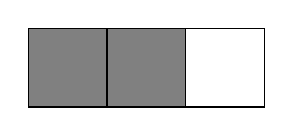
\begin{tikzpicture}
			\draw [draw=black] (3,1) rectangle (0,0);
			\draw [draw=black,fill=gray] (2,1) rectangle (0,0);
			\draw [] (1,1) -- (1,0);
			\draw [] (2,1) -- (2,0);
	\end{tikzpicture}}
	\caption{A relevant proposition.}\label{fig:relevant-p}
\end{subfigure}
\hfill
\begin{subfigure}[t]{.65\linewidth}
	\centering\scalebox{.8}{
		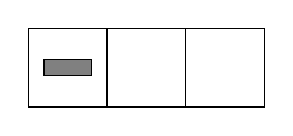
\begin{tikzpicture}
			\draw [draw=black] (3,1) rectangle (0,0);
			\draw [draw=black,fill=gray] (.8,.6) rectangle (.2,.4);
			\draw [] (1,1) -- (1,0);
			\draw [] (2,1) -- (2,0);
	\end{tikzpicture}}
	\hfill\scalebox{.8}{
		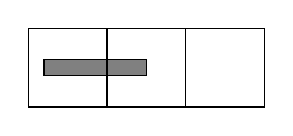
\begin{tikzpicture}
			\draw [draw=black] (3,1) rectangle (0,0);
			\draw [draw=black,fill=gray] (1.5,.6) rectangle (.2,.4);
			\draw [] (1,1) -- (1,0);
			\draw [] (2,1) -- (2,0);
	\end{tikzpicture}}\hfill\scalebox{.8}{
		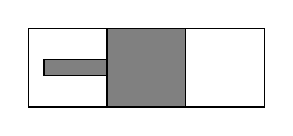
\begin{tikzpicture}
			\draw [draw=black] (3,1) rectangle (0,0);
			\draw [draw=black,fill=gray] (2,1) rectangle (1,0);
			\draw [draw=black,fill=gray] (1,.6) rectangle (.2,.4);
			\draw [] (1,1) -- (1,0);
			\draw [] (2,1) -- (2,0);
	\end{tikzpicture}}
	\caption{Irrelevant propositions.}\label{fig:over-p}
\end{subfigure}
\caption{Various QuD-proposition configurations (proposition defined by the gray area).}\label{fig:qud-p-diagrams}
\end{figure}

This notion is not sensitive to how the proposition at stake packages information: the only relevant(!) factor is whether or not the proposition as a whole can be identified with a union of cells. In other words, the level of granularity conveyed by the proposition is not taken into account when assessing its relevance to the question. This does not seem to match intuitions about what a relevant answer to a question is. For instance, the question set in (\ref{ex:relevant-answers}) strongly suggests a by-country partition of the CS.
\begin{exe}
\ex {In which country did Jo grow up?}
\begin{xlist}
	\ex[] {-- They grew up in France or Belgium.\hfill Relevant}\label{ex:relevant}
	\ex[??] {-- They grew up in Europe (for all I know). \hfill Relevant}\label{ex:relevant-coarse}
	\ex[?] {-- They grew up in Paris. \hfill Irrelevant (overinformative)}\label{ex:overinformative}
	\ex[?] {-- They grew up in Paris or Brussels. \hfill Irrelevant (overinformative)}\label{ex:overinformative-2}
	\ex[??] {-- They speak French natively \hfill More ``strongly'' irrelevant}\label{ex:irrelevant}
\end{xlist}
\label{ex:relevant-answers}
\end{exe}

Given this kind of partition, both (\ref{ex:relevant}) and (\ref{ex:relevant-coarse}) are predicted to be relevant, because France and Belgium are both countries and Europe is also a collection of countries. Yet, (\ref{ex:relevant-coarse}) does not seem so felicitous, at least without hedging. The oddness of this answer seem to come from the fact that \textit{Europe} is ``coarser-grained'' than, say, \textit{France or Belgium}. This can be modeled by saying \textit{Europe} can less straightforwardly be partitioned into country-level cells, than \textit{France or Belgium}. In fact, this is exactly the kind of intuition that Qtrees incorporate: a Qtree for \textit{France or Belgium} is predicted to have a country-level layer, with both \textit{France} and \textit{Belgium} flagged as verifying. A Qtree for \textit{Europe} would stop at the continent-level, the \textit{Europe}-node being verifying. Having a granularity-sensitive notion of Relevance may also help explain why finer-grained, overinformative answers like (\ref{ex:overinformative}) and (\ref{ex:overinformative-2}), are not so infelicitous: they suggest a partition of the CS whose cells (city-level) can all be mapped to a single (country-level) cell of the partition provided by the QuD. (\ref{ex:irrelevant}), which is also overinformative and predicted to be irrelevant, sounds more odd than (\ref{ex:overinformative}) and (\ref{ex:overinformative-2}), because the partition it suggests (\textit{What's Jo's level in French?}) cannot be properly mapped to the partition set by the QuD. For instance, Jo could very well be fluent in French, without having grown up in France. This suggests that granularity-sensitive notion of \textsc{Relevance} should state that a proposition is relevant if it can be partitioned into more specific ``sub-propositions'' (=verifying nodes), s.t. each sub-proposition ``fits'' a cell of the question, i.e., entails it.


We now introduce \textsc{Q-Relevance}, to incorporate a sightly weaker variant of this intuition. Our principle applies incrementally at each step of the Qtree computation process. \textsc{Q-Relevance} targets the verifying nodes of an input Qtree (which play the role of a ``structured'' proposition), and evaluates how these nodes ``fit'' into the output Qtree. A verifying node ``fits'' a Qtree iff it is not cut-out in this Qtree, i.e. iff there is no node of the Qtree that overlaps with it without fully containing it. In other words, no node of the output Qtree should \textit{strictly entail} a verifying node of the input Qtree. This is formalized in (\ref{ex:q-relevance}).

\begin{exe}
\ex {{\textsc{Q-Relevance}}.  Let $X$ and $Y$ be LFs and let $Qtrees(X)$ and $Qtrees(Y)$ be the sets of Qtrees compatible with $X$ and $Y$. Let $\circ$ be a Qtree-level operation, e.g. $\neg$, $\vee$, or $\rightarrow$. Let $C$ be a non-empty partial LF (incremental context). Two cases:
	\begin{itemize}
		\item $C=\circ$, with $\circ$ a unary operation. For any $T \in Qtrees(X)$, $\circ T$ is \textsc{Q-Relevant} with respect to $\circ X$ iff $\forall N \in \mathbb{N}^+(T). \ \neg\exists N' \in \mathbb{N}(\circ T). \ N' \subset N$.
		\item $C = X \circ$, with $\circ$ a binary operation. For any $T \in Qtrees(Y)$, $T_X \circ T_Y$ is \textsc{Q-Relevant} with respect to $X \circ Y$ iff $\forall N \in \mathbb{N}^+(T_Y). \ \neg\exists N' \in \mathbb{N}(T_x \circ T_Y). \ N' \subset N$.
\end{itemize}}\label{ex:q-relevance}
\end{exe}

The predictions of \textsc{Q-Relevance} for our $\lbrace \neg, \vee, \rightarrow\rbrace$ fragment of the language are the following. First, because $\neg$ is structure preserving, we can be sure that all the input verifying nodes are part of the negated output Qtree, satisfying \textsc{Q-Relevance}. Second, because $\vee$ forces well-formed unions of Qtrees (in terms of both structure and verifying nodes), we can be sure that all the input verifying nodes are part of the disjunctive output Qtree, again, satisfying \textsc{Q-Relevance}. The interesting cases arise with $\rightarrow$, because this operation involves intersecting verifying nodes and Qtrees, i.e. performing operations of the form $N \cap T$, with $N$ a verifying node of an antecedent Qtree, and $T$ a consequent Qtree. This kind of operation may affect the nodes of $T$ (in particular, $T$'s verifying nodes) in ways that may violate \textsc{Q-Relevance}. To see this, let us consider a Qtree $T_X\rightarrow T_Y$ compatible with an LF $X \rightarrow Y$. Within $T_X\rightarrow T_Y$, let us focus on a subtree $N\cap T_Y$, with $N \in \mathbb{N}^+(T_X)$. \textsc{Q-Relevance} imposes that for each verifying node in $T_Y$, no node of $N\cap T_Y$ strictly entails it: $\forall N' \in \mathbb{N}^+(T_Y). \neg \exists N'' \in \mathbb{N}(N\cap T_Y). \ N'' \subset N'$. If $N'$ in this formula is incompatible with $N$, then for sure no node $N''$ will strictly entail it. If $N'$ is compatible with $N$, then a violation of \textsc{Q-Relevance} arises as soon as $N \cap N' \subset N'$, i.e. if intersecting $N'$ with $N$ ``shrinks'' $N'$. This holds for any subtree $N\cap T_Y$ of $T_X\rightarrow T_Y$, with $N \in \mathbb{N}^+(T_X)$. Zooming out, this implies that each verifying node of the consequent Qtree compatible with some verifying node of the antecedent Qtree, should be fully preserved in the output.\\

We are now equipped to explain the oddness pattern of the HCs in (\ref{ex:hc}), whose Qtrees are repeated below. \textsc{Q-Relevance} predicts all the Qtrees compatible with the infelicitous HC (\ref{ex:hc-sw}) (cf. Figure \ref{fig:qtrees-if-not-noto-italy}) to be \textsc{Irrelevant}. This is because in each case, the output Qtree contains nodes that strictly entail the verifying \textit{Italy} node of the consequent Qtree: nodes of the form \textit{Italy and not Noto} (in Trees \ref{fig:tree-hc-sw-polar-polar-2} and \ref{fig:tree-hc-sw-polar-wh-2}), or city-level nodes (in Trees \ref{fig:tree-hc-sw-wh-2} and \ref{fig:qtree-if-not-noto-italy-tiered-wh-2}). (\ref{ex:hc-sw}) is thus predicted to be odd, in a way that is consistent with the intuition that raising \textit{Italy} after assuming \textit{not Noto} feels irrelevant to the general question the sentence is trying to answer.

\begin{figure}[H]
\centering
\setlength{\fboxsep}{1pt}
\renewcommand\thefigure{\ref{fig:qtrees-if-not-noto-italy}}
\begin{subfigure}[b]{.22\linewidth}
	\centering
	\scalebox{.7}
	{\begin{forest}for tree={s sep=2mm, inner sep=0, l=0}
			[CS [{Noto}] [{$\neg$Noto} [\fbox{\begin{tabular}{c}
					Italy$\cap\neg$Noto\\
					\textbf{\textcolor{red}{$\subset$ Italy}}
			\end{tabular}}][$\neg$Italy]]]
	\end{forest}}
	\caption{Tree \ref{fig:qtree-not-noto-polar} $\rightarrow$ Tree \ref{fig:qtree-italy-polar}.}\label{fig:tree-hc-sw-polar-polar-2}
\end{subfigure}\hfill
\begin{subfigure}[b]{.22\linewidth}
	\centering
	\scalebox{.7}
	{\begin{forest}for tree={s sep=2mm, inner sep=0, l=0}
			[CS [{Noto}] [{$\neg$Noto} [\fbox{\begin{tabular}{c}
					Italy$\cap\neg$Noto\\
					\textbf{\textcolor{red}{$\subset$ Italy}}
			\end{tabular}}][France] [...]]]
	\end{forest}}
	\caption{Tree \ref{fig:qtree-not-noto-polar} $\rightarrow$ Tree \ref{fig:qtree-italy-wh}.}\label{fig:tree-hc-sw-polar-wh-2}
\end{subfigure}\hfill
\begin{subfigure}[b]{.3\linewidth}
	\centering
	\scalebox{.7}
	{\begin{forest}for tree={s sep=2mm, inner sep=0, l=0}
			[CS [{Noto}] [\fbox{\begin{tabular}{c}
					Rome\\
					\textbf{\textcolor{red}{$\subset$ Italy}}
			\end{tabular}}] [\fbox{\begin{tabular}{c}
					...\\
					\textbf{\textcolor{red}{$\subset$ Italy}}
			\end{tabular}}] [{Paris}] [...]]
	\end{forest}}
	\caption{Tree \ref{fig:qtree-not-noto-wh} $\rightarrow$ Tree \ref{fig:qtree-italy-wh}/\ref{fig:qtree-italy-polar}.}\label{fig:qtree-if-not-noto-italy-wh-wh-2}\label{fig:tree-hc-sw-wh-2}
\end{subfigure}\hfill
\begin{subfigure}[b]{.25\linewidth}
	\centering
	\scalebox{.7}
	{\begin{forest}for tree={s sep=2mm, inner sep=0, l=0}
			[CS [Italy[{Noto}] [\fbox{\begin{tabular}{c}
					Rome\\
					\textbf{\textcolor{red}{$\subset$ Italy}}
			\end{tabular}}] [\fbox{\begin{tabular}{c}
					...\\
					\textbf{\textcolor{red}{$\subset$ Italy}}
			\end{tabular}}]]  [...]]
	\end{forest}}
	\caption{Tree \ref{fig:qtree-not-noto-tiered} $\rightarrow$ Tree \ref{fig:qtree-italy-wh}/\ref{fig:qtree-italy-polar}.}\label{fig:qtree-if-not-noto-italy-tiered-wh-2}
\end{subfigure}
\caption{Qtrees for (\ref{ex:hc-sw})=\#\textit{If SuB29 will not take place in Noto, it will take place in Italy.}}
\end{figure}

Regarding the felicitous HC (\ref{ex:hc-ws}), \textsc{Q-Relevance} predicts some, but crucially not all, of the Qtrees in Figure \ref{fig:qtrees-if-italy-not-noto} to be \textsc{Irrelevant}. Trees \ref{ex:qtree-if-italy-not-noto-polar-polar-2} and \ref{ex:qtree-if-italy-not-noto-wh-polar-2} are \textsc{Irrelevant}, because in both cases, the output Qtree contains nodes of the form \textit{Italy and not Noto}, which strictly entail the verifying \textit{not Noto} node of the consequent Qtree. Trees \ref{ex:qtree-if-italy-not-noto-polar-wh-2} and \ref{ex:qtree-if-italy-not-noto-wh-wh-2} however, do not violate \textsc{Q-Relevance}, because they are constructed from a consequent Qtree for \textit{not Noto} that introduces a city-level partition that perfectly ``fits'' the restriction to \textit{Italy} introduced by the antecedent Qtree, so that no city-node verifying \textit{not Noto} is strictly entailed by a node in the output Qtree. This correctly predicts (\ref{ex:hc-ws}) to be felicitous, in a way that is consistent with the intuition that it is possible to make sense of \textit{not Noto} after assuming \textit{Italy}, granted that \textit{not Noto} discusses a \textit{which city?} kind of question.



\begin{figure}[H]
\setlength{\fboxsep}{1pt}
\renewcommand\thefigure{\ref{fig:qtrees-if-italy-not-noto}}
\centering
\begin{subfigure}[b]{.23\linewidth}
	\centering
	\scalebox{.8}
	{\begin{forest}for tree={s sep=2mm, inner sep=0, l=0}
			[CS [{Italy} [Noto][\fbox{\begin{tabular}{c}
					$\neg$Noto$\cap$Italy\\
					\textbf{\textcolor{red}{$\subset \neg$Noto}}
			\end{tabular}}]] [{$\neg$Italy} ]]
	\end{forest}}
	\caption{Tree \ref{fig:qtree-italy-polar} $\rightarrow$ Tree \ref{fig:qtree-not-noto-polar}.}\label{ex:qtree-if-italy-not-noto-polar-polar-2}
\end{subfigure}\hfill
\begin{subfigure}[b]{.25\linewidth}
	\centering
	\scalebox{.8}
	{\begin{forest}for tree={s sep=2mm, inner sep=0, l=0}
			[CS [{Italy} [{Noto}] [\fbox{Rome}] [\fbox{...}]] [{$\neg$Italy} ]]
	\end{forest}}
	\caption{Tree \ref{fig:qtree-italy-polar} $\rightarrow$ Tree \ref{fig:qtree-not-noto-wh}/\ref{fig:qtree-not-noto-tiered}.}\label{ex:qtree-if-italy-not-noto-polar-wh-2}
\end{subfigure}
\hfill
\begin{subfigure}[b]{.25\linewidth}
	\centering
	\scalebox{.8}
	{\begin{forest}for tree={s sep=2mm, inner sep=0, l=0}
			[CS [Italy[Noto][\fbox{\begin{tabular}{c}
					$\neg$Noto$\cap$Italy\\
					\textbf{\textcolor{red}{$\subset \neg$Noto}}
			\end{tabular}}]] [France] [...]]
	\end{forest}}
	\caption{Tree \ref{fig:qtree-italy-wh} $\rightarrow$ Tree \ref{fig:qtree-not-noto-polar}.}\label{ex:qtree-if-italy-not-noto-wh-polar-2}
\end{subfigure}\hfill
\begin{subfigure}[b]{.25\linewidth}
	\centering
	\scalebox{.8}
	{\begin{forest}for tree={s sep=2mm, inner sep=0, l=0}
			[CS [Italy[{Noto}] [\fbox{Rome}] [\fbox{...}]] [France] [...] ]
	\end{forest}}
	\caption{Tree \ref{fig:qtree-italy-wh} $\rightarrow$ Tree \ref{fig:qtree-not-noto-wh}/\ref{fig:qtree-not-noto-tiered}.}\label{ex:qtree-if-italy-not-noto-wh-wh-2}
\end{subfigure}
\caption{Qtrees for (\ref{ex:hc-ws})=\textit{If SuB29 will take place in Italy, it will not take place in Noto.}}\label{ex:qtree-if-italy-not-noto-2}
\end{figure}

\section{Extensions}\label{sec:ccl}
We developed an account of Hurford Sentences based on implicit QuDs and constraints on their derivation. This framework captured the challenging contrast between HDs, which are infelicitous regardless of the order of the disjuncts, and HCs, whose felicity profile seems sensitive to granularity considerations. We also sketched how this model could capture Long-Distance HDs.

\subsection{Compatible, non-entailing disjuncts}


Interestingly, the model extends its scope to HDs with merely compatible disjuncts \citep{Singh2008b}, exemplified in (\ref{ex:hd-compatible}).

\begin{exe}
\ex[\#] {SuB29 will take place in the Basque country\footnotemark{} or France.}\label{ex:hd-compatible}
\end{exe} 
\footnotetext{Given that the Basque country encompasses Northern Central Spain and southwestern France, it is compatible with \textit{France}, without entailment in any direction.}

In (\ref{ex:hd-compatible}) the first disjunct suggests a by-region partition, such that the Basque country represents a (verifying) leaf; while the second disjunct suggests a by-country partition, such that France represents a (verifying) leaf. The relevant Qtrees are built in Figure \ref{fig:qtrees-compat}.

\begin{figure}[H]
\centering
\begin{subfigure}[b]{.55\linewidth}
	\centering
	\scalebox{.8}{
		\begin{forest}for tree={s sep=2mm, inner sep=0, l=0}
			[CS [\fbox{Basque}] [$\neg${Basque}]]
	\end{forest}}
	\hfill
	\scalebox{.8}{
		\begin{forest}for tree={s sep=2mm, inner sep=0, l=0}
			[CS [\fbox{Basque country}] [Navarre] [Midi] [...]]
	\end{forest}}
	\caption{Qtrees for \textit{SuB29 will take place in the Basque country}, given principles (\ref{ex:qtree-simplex-def}\ref{pt:simplex-qtree-polar}) (left tree) or (\ref{ex:qtree-simplex-def}\ref{pt:simplex-qtree-wh}) (right tree).}\label{fig:qtrees-basque}
\end{subfigure}\hfill
\begin{subfigure}[b]{.4\linewidth}
	\centering
	\scalebox{.8}{
		\begin{forest}for tree={s sep=2mm, inner sep=0, l=0}
			[CS [\fbox{France}] [$\neg$France]]
	\end{forest}}\hfill
	\scalebox{.8}{
		\begin{forest}for tree={s sep=2mm, inner sep=0, l=0}
			[CS [\fbox{France}] [Spain] [...]]
	\end{forest}}
	\caption{Qtrees for \textit{SuB29 will take place in France}, given principles (\ref{ex:qtree-simplex-def}\ref{pt:simplex-qtree-polar}) (left tree) or (\ref{ex:qtree-simplex-def}\ref{pt:simplex-qtree-wh}) (right tree).}\label{fig:qtrees-france}
\end{subfigure}\hfill
\caption{Possible Qtrees for the disjuncts of (\ref{ex:hd-compatible}).}\label{fig:qtrees-compat}
\end{figure}


Can  a disjunctive Qtree be built for (\ref{ex:hd-compatible})? It turns out that the trees in Figure \ref{fig:qtrees-basque} cannot be properly disjoined with any of those in Figure \ref{fig:qtrees-france}, due to the fact that they introduce different, parallel partitionings. The only remaining way to disjoin Qtrees associated with each disjunct of (\ref{ex:hd-compatible}), would be to create a tiered Qtree for \textit{SuB29 will take place in the Basque country}, involving a by-country layer (\textit{via} principle (\ref{ex:qtree-simplex-def}\ref{pt:simplex-qtree-tiered})). But a problem arises in the formation of such a Qtree. Given that \textit{p}=\textit{SuB29 will take place in the Basque country} does not entail that SuB29 will place in any single specific country, it is impossible to create a $p$-chain containing a country-level alternative to $p$. Consequently, no Qtree generated from \textit{SuB29 will take place in the Basque country} using principle (\ref{ex:qtree-simplex-def}\ref{pt:simplex-qtree-tiered}) will contain a by-country layer. To summarize, we predict a sentence like (\ref{ex:hd-compatible}) to be odd because it features compatible disjuncts with incomparable degrees of granularity, which cannot lead to any well-formed disjunctive Qtree.

However, HC-variants of (\ref{ex:hd-compatible}) are predicted by our model to be odd regardless of the ordering of the antecedent and consequent, because Qtrees evoked by \textit{France} and Qtrees evoked by \textit{the Basque country} are not in any kind of refinement relation. This prediction is not empirically borne out, as shown in (\ref{ex:hc-compatible}).

\begin{exe}
\ex \label{ex:hc-compatible}
\begin{xlist}
	\ex[?] {If SuB29 will take place in France, it will take place in the Basque country.}\label{ex:hc-compatible-ws}
	\ex[\#] {If SuB29 will take place in the Basque country, it will take place in France.}\label{ex:hc-compatible-sw}
\end{xlist}
\end{exe}

Within our framework, the contrast in (\ref{ex:hc-compatible}) suggests that it is somehow easier to split the set of \textit{Basque country} worlds into French and Spanish subsets (in order to satisfy \textsc{Q-Relevance} in \ref{ex:hc-compatible-ws}), than to split the set of \textit{France} worlds into Basque and non-Basque subsets (in order to satisfy \textsc{Q-Relevance} in \ref{ex:hc-compatible-sw}). Future work should investigate when, and how such coercion operations on Qtrees can take place.\\





\iffalse
\begin{subfigure}[b]{.33\linewidth}
\centering
\scalebox{.8}{
	\begin{forest}for tree={s sep=7mm, inner sep=0, l=0}
		[CS [{France} [Midi] [~]] [Spain [~] [Navarre]] [...]]
		\node[draw,align=center] at (-.75,-2.3) {Basque\\country};
\end{forest}}
\caption{A tentative Qtree for \textit{Sub will take place in the Basque country}, given principle (\ref{ex:qtree-simplex-def}\ref{pt:simplex-qtree-tiered})}\label{fig:qtree-basque-tiered}
\end{subfigure}
\fi

\subsection{``Long-Distance'' HCs}
In this section, we explore how our QuD-informed view of redundancy captures two kinds of ``Long-Distance'' variants of HCs: those derived from LDHDs \textit{via} the \textit{or-to-if} tautology; and those derived by applying the ``Long Distance'' recipe directly to HCs. 


\subsubsection{LDHCs derived from LDHDs}

Recall that ``Long Distance'' HDs (\textbf{LDHDs}, \citenp{Marty2022}) are obtained from standard HDs of the form \p{} $\vee$ \pplus{} by further disjoining \pplus{} with a proposition \r{}, s.t. \pplus{} $\vee$ \r{} is not redundant, and no longer entails \p. This can be done by choosing \r{} to contradict \pplus{} and \p{}. Such constructions have been argued to be deviant, despite the fact that none of their disjuncts are in an entailment relation (and thus satisfy the traditional, non-explanatory version of Hurford's Constraint). (\ref{ex:ldhd-pos}) illustrates a classic LDHD: \textit{Europe} entails \textit{France}, and \textit{France} is further disjoined with \textit{New York}, that is incompatible with \textit{Europe} -- making the two main disjuncts compatible, but non-entailing.  (\ref{ex:ldhd-neg}) illustrates a perhaps more degenerate case of LDHD: the weak disjunct, \textit{not France}, takes the form of the negation of the stronger disjunct of (\ref{ex:ldhd-pos}); the stronger disjunct, \textit{not Europe}, takes the form of the negation of the weak disjunct of (\ref{ex:ldhd-pos}); and the extra proposition disjoined with it (\textit{Paris}), is chosen to be incompatible with \textit{not France} and \textit{not Europe}. Note that the kind of variable change we described here, was already used to construct simple infelicitous HCs like (\ref{ex:hc-ns-w}).

\begin{exe}
	\exr{ex:ldhd}
	\begin{xlist}
		\ex[\#] {Jo either studied in \textcolor{blue}{Europe}, or in \textcolor{orange}{France} or in \textcolor{green}{New York}.
			\hfill \p{} $\vee$ (\pplus{} $\vee$ \r)}\label{ex:ldhd-pos}
		\ex[\#] {Jo either does\textcolor{blue}{n't study in France}, or \textcolor{orange}{not in Europe} or in \textcolor{green}{Paris}.	\hfill \textbf{\textcolor{blue}{q}} $\vee$ (\textcolor{orange}{\textbf{q}$^+$} $\vee$ \r)\\
			with: \textbf{\textcolor{blue}{q}} := $\neg$\pplus; \textcolor{orange}{\textbf{q}$^+$} := $\neg$\p }\label{ex:ldhd-neg}
	\end{xlist}
\end{exe}

We think that both (\ref{ex:ldhd-pos}) and (\ref{ex:ldhd-neg}) are degraded -- which is in itself interesting because SR predicts (\ref{ex:ldhd-neg}) to be fine.

\begin{exe}
	\ex 
	\begin{xlist}
		\ex {(\ref{ex:ldhd-pos})=\p{} $\vee$ (\pplus{} $\vee$ \r) is SR.\\
			C = \pplus. $\forall D. $ \p{} $\vee$ ((\pplus{}$\wedge$ $D$) $\vee$ \r) $\equiv$ \p{} $\vee$ ((\pplus{}$\vee$ \r) $\wedge$ ($D$ $\vee$ \r)) $\equiv$ (\p{} $\vee$ \r) $\wedge$ (\p{} $\vee$ $D$ $\vee$ \r) $\equiv$ \p{} $\vee$ \r}
		\ex {(\ref{ex:ldhd-neg}) = $\neg$\pplus{} $\vee$ ($\neg$\p{} $\vee$ \r) is not SR.\\
			C = $\neg$\pplus. Take $D = \top$.\\
			$\neg$(\pplus{} $\wedge$ $D$) $\vee$ ($\neg$\p{} $\vee$ \r) $\equiv$ $\neg$\pplus{} $\vee$ ($\neg$\p{} $\vee$ \r) $\equiv$ $\neg$\pplus{} $\vee$ \r{} $\not\equiv$ $\neg$\p{} $\vee$ \r\\
			C = $\neg$\p. Take $D = \bot$.\\
			$\neg$\pplus{} $\vee$ ($\neg$(\p{} $\wedge$ $D$) $\vee$ \r) $\equiv$ $\neg$\pplus{} $\vee$ ($\top$ $\vee$ \r) $\equiv$ $\top$ $\not\equiv$ $\neg$\pplus{} $\vee$ \r\\
			C = \r. Take $D = \top$.\\
			$\neg$\pplus{} $\vee$ ($\neg$\p{} $\vee$ (\r{} $\wedge$ $D$)) $\equiv$ $\neg$\pplus{} $\vee$ \r{} $\not\equiv$ $\neg$\pplus $\equiv$ $\neg$\pplus{} $\vee$ $\neg$\p{}\\
			C = ($\neg$\p{} $\vee$ \r). Take $D = \top$.\\
			$\neg$\pplus{} $\vee$ (($\neg$\p{} $\wedge$ $D$) $\vee$ (\r{} $\wedge$ $D$)) $\equiv$ $\neg$\pplus{} $\vee$ ($\neg$\p{} $\vee$ \r) $\equiv$ $\neg$\pplus{} $\vee$ \r{} $\not\equiv$ $\neg$\pplus
			
		}
	\end{xlist}
	
\end{exe}

Interestingly, turning the LDHDs in (\ref{ex:ldhd}) into conditionals maintains infelicity, as shown in (\ref{ex:ldhc}).

\begin{exe}
	\exr{ex:ldhc}
	\begin{xlist}
		\ex[\#] {If Jo did not study in \textcolor{blue}{Europe}, she studied in \textcolor{orange}{France} or in \textcolor{green}{New York}.}
		\ex[\#] {If Jo studied in \textcolor{blue}{France}, she did not study \textcolor{orange}{in Europe} or she studied in \textcolor{green}{Paris}.}
	\end{xlist}
\end{exe}

We proceed to show that both (\ref{ex:ldhc-pos}) and (\ref{ex:ldhc-neg}) are \textsc{Q-Redundant}. \textsc{Q-Redundancy}, as defined in Chapter \ref{chap:hurford-sentences}, states that a Qtree $T$ paired with a specific LF $X$ is deviant iff the $T$ is equivalent to a tree $T'$ compatible with a simplification of $X$. (\ref{ex:ldhc-pos}) is then \textsc{Q-Redundant} because any Qtree it evokes is also evoked by (\ref{ex:ldhc-pos-simplification}); and (\ref{ex:ldhc-neg}) is \textsc{Q-Redundant} as well, because any Qtree it evokes is also evoked by (\ref{ex:ldhc-neg-simplification}).

\begin{exe}
	\ex\label{ex:ldhc-simplifications}
	\begin{xlist}
		\ex[] {If Jo did not study in \textcolor{blue}{Europe}, she studied in \textcolor{green}{New York}.}\label{ex:ldhc-pos-simplification}
		\ex[] {If Jo studied in \textcolor{blue}{France}, she studied in \textcolor{green}{Paris}.}\label{ex:ldhc-neg-simplification}
	\end{xlist}
\end{exe}

We start with (\ref{ex:ldhc-pos}). The possible Qtrees evoked by its antecedent ($\neg$\textit{Europe}) are depth-1 Qtrees whose leaves are $\lbrace$\textit{Europe}, $\neg$\textit{Europe}$\rbrace$, or continent-level alternatives $\lbrace$\textit{Europe}, \textit{Africa}, \textit{Asia}, ...$\rbrace$. ``Tiered'' Qtrees are unlikely, since coarser-grained alternatives to continent-level locations are themselves unlikely to be salient. In each possible Qtree, the leaves incompatible with \textit{Europe} are flagged as verifying (effect of negation). This is summarized in Figure \ref{trees:not-Europe}.

\begin{figure}[H]
	\centering
	\begin{subfigure}[b]{.3\linewidth}
		\centering
		\scalebox{1}{
			\begin{forest}
				[CS[Europe][\fbox{$\neg$Europe}]]
			\end{forest}
		}
		\caption{}\label{tree:not-europe-polar}
	\end{subfigure}
	\qquad
	\begin{subfigure}[b]{.3\linewidth}
		\centering
		\scalebox{1}{
			\begin{forest}
				[CS[Europe][\fbox{America}][\fbox{Africa}][\fbox{...}]]
			\end{forest}
		}
		\caption{}\label{tree:not-europe-wh}
	\end{subfigure}
	\caption{Qtrees for \textit{Jo did not study in \textcolor{blue}{\textbf{Europe}}.}}\label{trees:not-Europe}
\end{figure}

The consequent of (\ref{ex:ldhc-pos}) is disjunctive, and therefore results from the well-formed union of Qtrees evoked by its two disjuncts (\textit{France} and \textit{New York}). Possible Qtrees for \textit{France} (already computed in section \ref{sec:qtrees-scalemates-non-scalemates}), are repeated in Figure \ref{trees:france-2}; possible Qtrees for \textit{New York} can be computed in a way that is strictly analogous to Qtrees for \textit{Paris} (as done in section \ref{sec:qtrees-scalemates-non-scalemates}), and are thus given in Figure \ref{trees:new-york}.
\begin{figure}[H]
	\centering
	\begin{subfigure}[b]{.3\linewidth}
		\centering
		\begin{forest}
			[CS[\bfbox{France}][$\neg$France]]
		\end{forest}
		\caption{}\label{tree:france-polar-2}
	\end{subfigure}
	\qquad
	\begin{subfigure}[b]{.3\linewidth}
		\centering
		\begin{forest}
			[CS[\bfbox{France}][US][...]]
		\end{forest}
		\caption{}\label{tree:france-wh-2}
	\end{subfigure}
	\caption{Qtrees for \textit{Jo studied in \textbf{\textcolor{blue}{France}}}.} \label{trees:france-2}
\end{figure}

\begin{figure}[H]
	\centering
	\begin{subfigure}[b]{.3\linewidth}
		\centering
		\scalebox{1}{
			\begin{forest}
				for tree={s sep=2mm, inner sep=0, l=0}
				[CS[\gfbox{New York}][$\neg$New York]]
		\end{forest}}
		\caption{}\label{tree:new-york-polar}
	\end{subfigure}
	\hfill
	\begin{subfigure}[b]{.3\linewidth}
		\centering
		\scalebox{1}{
			\begin{forest}
				for tree={s sep=2mm, inner sep=0, l=0}
				[CS[\gfbox{New York}][Boston][Paris][...]]
		\end{forest}}
		\caption{}\label{tree:new-york-wh}
	\end{subfigure}\hfill
	\begin{subfigure}[b]{.3\linewidth}
		\centering
		\scalebox{1}{
			\begin{forest}
				for tree={s sep=2mm, inner sep=0, l=0}
				[CS[France[{Paris}][...]][US[\gfbox{New York}][Boston]][...]]
		\end{forest}}
		\caption{}\label{tree:new-york-tiered}
	\end{subfigure}
	
	
	\caption{Qtrees for \textit{Jo studied in \textbf{\textcolor{green}{New York}}.}}\label{trees:new-york}
\end{figure}

Unioning Qtrees from Figures \ref{trees:france-2} and \ref{trees:new-york} can be done in only one way: using Tree \ref{tree:france-wh-2} for \textit{France}, and Tree \ref{tree:new-york-tiered}, for \textit{New York}. This yields the Qtree in Figure \ref{tree:france-or-new-york}.

\begin{figure}[H]
	\centering
	\scalebox{1}{
		\begin{forest}
			for tree={s sep=2mm, inner sep=0, l=0}
			[CS[\fbox{France}[{Paris}][...]][US[\fbox{New York}][Boston][...]][...]]
	\end{forest}}
	\caption{Qtree for \textit{Jo studied in \textcolor{orange}{\textbf{France}} or in \textcolor{green}{\textbf{New York}}}.}\label{tree:france-or-new-york}
\end{figure}

Now that Qtrees for the antecedent and the consequent of (\ref{ex:ldhc-pos}) are derived, we can combine them to form a Qtree for the whole conditional, by taking the antecedent Qtrees from Figure \ref{trees:not-Europe} and replacing their verifying nodes (anything non Europe) by their intersection with the consequent Qtree from Figure \ref{tree:france-or-new-york}. This yields the Qtrees in Figure \ref{trees:if-not-Europe-then-france-or-new-york}. 

\begin{figure}[H]
	\centering
	\begin{subfigure}[b]{.45\linewidth}
		\centering
		\scalebox{1}{
			\begin{forest}
				for tree={s sep=2mm, inner sep=0, l=0}
				[CS[Europe][{$\neg$Europe} [US[\fbox{New York}][Boston][...]][Japan[...]][...]]]
			\end{forest}
		}
		\caption{}
	\end{subfigure}
	\hfill
	\begin{subfigure}[b]{.45\linewidth}
		\centering
		\scalebox{1}{
			\begin{forest}
				for tree={s sep=2mm, inner sep=0, l=0}
				[CS[Europe][{America}[US[\fbox{New York}][Boston][...]][...]][{Africa}[...]][{...}]]
			\end{forest}
		}
		\caption{}
	\end{subfigure}
	\caption{Qtrees for (\ref{ex:ldhc-pos}) = \textit{If Jo did not study in \textcolor{blue}{\textbf{Europe}}, she studied in \textcolor{orange}{\textbf{France}} or in \textcolor{green}{\textbf{New York}}.}}\label{trees:if-not-Europe-then-france-or-new-york}
\end{figure}

Crucially, the intersection operation between the consequent Qtree in Figure \ref{tree:france-or-new-york}, and the non-Europe nodes in the Qtrees from Figure \ref{trees:not-Europe}, discarded the sections of the consequent Qtree that had to do with \textit{France}. This does not violate \textsc{Q-Relevance}, but instead, causes the output Qtrees to be identical (and hence, equivalent) to Qtrees evoked by a formal simplification of (\ref{ex:ldhc-pos}) that does not feature \textit{France} as a disjunct in its consequent -- namely, (\ref{ex:ldhc-pos-simplification}). Any Qtree derived from (\ref{ex:ldhc-pos}) is thus \textsc{Q-Redundant}, and as a result, we correctly predict (\ref{ex:ldhc-pos}) to be infelicitous.\\

We can now move on to the case of (\ref{ex:ldhc-neg}). The possible Qtrees evoked by its antecedent (France), are already given in Figure \ref{trees:france-2}.


The consequent of (\ref{ex:ldhc-neg}) is disjunctive, and therefore results from the well-formed union of Qtrees evoked by its two disjuncts ($\neg$\textit{Europe} and \textit{Paris}). Possible Qtrees for $\neg$\textit{Europe} are already given in Figure \ref{trees:not-Europe}. Possible Qtrees for \textit{Paris} are given in Figure \ref{trees:paris}.

\begin{figure}[H]
	\centering
	\begin{subfigure}[b]{.3\linewidth}
		\centering
		\scalebox{1}{
			\begin{forest}
				for tree={s sep=2mm, inner sep=0, l=0}
				[CS[\ofbox{Paris}][$\neg$Paris]]
		\end{forest}}
		\caption{}\label{tree:paris-polar}
	\end{subfigure}
	\hfill
	\begin{subfigure}[b]{.3\linewidth}
		\centering
		\scalebox{1}{
			\begin{forest}
				for tree={s sep=2mm, inner sep=0, l=0}
				[CS[\ofbox{Paris}][Nice][London][...]]
		\end{forest}}
		\caption{}\label{tree:paris-wh}
	\end{subfigure}\hfill
	\begin{subfigure}[b]{.3\linewidth}
		\centering
		\scalebox{1}{
			\begin{forest}
				for tree={s sep=2mm, inner sep=0, l=0}
				[CS[France[\ofbox{Paris}][Nice][...]][UK[London][...]][...]]
		\end{forest}}
		\caption{}\label{tree:paris-tiered}
	\end{subfigure}
	\begin{subfigure}[b]{.3\linewidth}
		\centering
		\scalebox{1}{
			\begin{forest}
				for tree={s sep=2mm, inner sep=0, l=0}
				[CS[Europe[France[\fbox{Paris}][Nice][...]][UK[London][...]]][America[...]][...]]
		\end{forest}}
		\caption{}\label{tree:paris-tiered-tiered}
	\end{subfigure}
	
	
	\caption{Qtrees for \textit{Jo studied in \textbf{\textcolor{orange}{Paris}}.}}\label{trees:paris}
\end{figure}

Unioning Qtrees from Figures \ref{trees:not-Europe} and \ref{trees:paris} can be done in only one way: using Tree \ref{tree:not-europe-wh} for $\neg$\textit{Europe}, and Tree \ref{tree:paris-tiered-tiered}, for \textit{Paris}. This yields the Qtree in Figure \ref{tree:not-europe-or-paris}.

\begin{figure}[H]
	\centering
	\scalebox{1}{
		\begin{forest}
			for tree={s sep=2mm, inner sep=0, l=0}
			[CS[Europe[France[\fbox{Paris}][Nice][...]][UK[London][...]]][\fbox{America}[{...}]][\fbox{...}]]
	\end{forest}}
	\caption{Qtrees for \textit{Jo did not study in \textbf{\textcolor{blue}{Europe}} or studied in \textbf{\textcolor{orange}{Paris}}.}}\label{tree:not-europe-or-paris}
\end{figure}

Now that Qtrees for the antecedent and the consequent of (\ref{ex:ldhc-neg}) are derived, we can combine them to form a Qtree for the whole conditional, by taking the antecedent Qtrees from Figure \ref{trees:france-2} and replacing their verifying nodes (\textit{France} nodes) by their intersection with the consequent Qtree from Figure \ref{tree:not-europe-or-paris}. This yields the Qtrees in Figure \ref{trees:if-france-then-not-europe-or-paris}. 

\begin{figure}[H]
	\centering
	\begin{subfigure}[b]{.3\linewidth}
		\centering
		\begin{forest}
			[CS[{France}[\fbox{Paris}][Nice][...]][$\neg$France]]
		\end{forest}
		\caption{}
	\end{subfigure}
	\qquad
	\begin{subfigure}[b]{.3\linewidth}
		\centering
		\begin{forest}
			[CS[{France}[\fbox{Paris}][Nice][...]][US][...]]
		\end{forest}
		\caption{}
	\end{subfigure}
	\caption{Qtrees for (\ref{ex:ldhc-neg}) = \textit{If Jo studied in \textcolor{blue}{\textbf{France}}, she did not study in \textcolor{orange}{\textbf{Europe}} or she studied in \textcolor{green}{\textbf{Paris}}.}} \label{trees:if-france-then-not-europe-or-paris}
\end{figure}

Crucially, the intersection operation between the consequent Qtree in Figure \ref{tree:not-europe-or-paris}, and the \textit{France} nodes in the Qtrees from Figure \ref{trees:france-2}, discarded the sections of the consequent Qtree that had to do with $\neg$\textit{Europe}. This does not violate \textsc{Q-Relevance}, but instead, causes the output Qtrees to be identical (and hence, equivalent) to Qtrees evoked by a formal simplification of (\ref{ex:ldhc-neg}) that does not feature $\neg$\textit{Europe} as a disjunct in its consequent -- namely, (\ref{ex:ldhc-neg-simplification}). Any Qtree derived from (\ref{ex:ldhc-neg}) is thus \textsc{Q-Redundant}, and as a result, we correctly predict (\ref{ex:ldhc-neg}) to be infelicitous.\\

In sum, \textsc{Q-Redundancy} predicts both kinds of LDHCs derived from LDHDs via the \textit{or-to-if} tautology to be infelicitous, in line with pre-theoretical intuitions about these sentences.




\subsubsection{LDHCs derived from HCs}

This reasoning extends to the LDHCs (\ref{ex:ldhc-w-ns}) and (\ref{ex:ldhc-ns-w}), whose trees are given in Fig. \ref{fig:ldhc-non-scalar-w-ns} and \ref{fig:ldhc-non-scalar-ns-w}. For (\ref{ex:ldhc-w-ns}), \textsc{Q-Relevance} is satisfied because none of the verifying leaves from the consequent Qtree (cities different from Paris and Brussels) are cut across in the output Qtree. The feeling of redundancy in (\ref{ex:ldhc-w-ns}) may come from the fact removing \textit{Brussels} from the sentence leads to the same overall meaning and Qtree.\footnote{Following \citet{HenotMortier2024a,HenotMortier2024b}, this implies that (\ref{ex:ldhc-w-ns}) is \textsc{Q-Redundant}.} For (\ref{ex:ldhc-ns-w}), \textsc{Q-Relevance} is violated because the compatible \textit{France} leaf from the consequent Qtree cannot ``fit'' into the city-level nodes introduced by the antecedent.


\begin{minipage}{.45\linewidth}
	\centering
	\begin{figure}[H]
		\centering
		\scalebox{.7}{
			\begin{forest}
				[CS[FR[Paris][\fbox{Nice}][\fbox{...}]][$\neg$FR/UK]]
		\end{forest}}
		\caption{Qtree for (\ref{ex:ldhc-w-ns}).}\label{fig:ldhc-non-scalar-w-ns}
	\end{figure}
\end{minipage}
\hfill
\begin{minipage}{.45\linewidth}
	\centering
	\begin{figure}[H]
		\centering
		\scalebox{.7}{
			\begin{forest}
				[CS[Paris][Brussels][\fbox{\begin{tabular}{c}
						FR$\wedge$Nice\\
						\textcolor{red}{$\subset$ FR}
				\end{tabular}}][...]]
		\end{forest}}
		\caption{Qtree for (\ref{ex:ldhc-ns-w}).}\label{fig:ldhc-non-scalar-ns-w}
	\end{figure}
\end{minipage}





An argument against this view comes from Long-Distance HCs (henceforth LDHC). Such structures, inspired from Long-Distance HDs (\cite{Marty2022}) and exemplified in (\ref{ex:ldhc}), are derived from (\ref{ex:hc-s}) by further disjoining \pplus{} with a proposition \r{} taken to be incompatible with \p. 


\begin{exe}
	\ex\label{ex:ldhc-surface}
	\begin{xlist}
		\ex[?] {If Jo studied in \textcolor{blue}{France} she didn't study in \textcolor{orange}{Paris} or \textcolor{green}{Brussels}.\hfill \p$\rightarrow\neg$(\pplus$\vee$\r)}\label{ex:ldhc-w-ns}
		\ex[\#] {If Jo didn't study in \textcolor{orange}{Paris} or \textcolor{green}{Brussels} she studied in \textcolor{blue}{France}.\hfill $\neg$(\pplus$\vee$\r)$\rightarrow$\p}\label{ex:ldhc-ns-w}
	\end{xlist}
\end{exe}

Felicity-wise, LDHCs seem quite degraded: (\ref{ex:ldhc-w-ns}) is felt to convey the same kind of information twice (because having studied in France contextually entails not having studied in Brussels), while (\ref{ex:ldhc-ns-w})'s consequent feels independent from the subject matter raised by the antecedent. Yet neither (\ref{ex:ldhc-w-ns}) nor (\ref{ex:ldhc-ns-w}) are predicted to be SR, due to the presence of \r{}.

\begin{exe}
	\ex (\ref{ex:ldhc-w-ns}) is not SR
	\begin{xlist}
		\ex {C = \pplus{} $\vee$\r. Take $D = \top$.\\\p{} $\rightarrow$ $\neg$((\pplus{} $\vee$ \r) $\wedge$ $D$) $\equiv$ \p{} $\rightarrow$ $\neg$(\pplus{} $\vee$ \r) $\not\equiv$ \p}
		\ex {C = \p. Take $D = \bot$.\\
			(\p{} $\wedge$ $D$) $\rightarrow$ $\neg$(\pplus{}$\vee$ \r) $\equiv$ (\p{} $\wedge$ $\bot$) $\rightarrow$ $\neg$(\pplus{}$\vee$ \r) $\equiv$ $\bot$ $\rightarrow$ $\neg$(\pplus{}$\vee$ \r) $\equiv$ $\top$ $\not\equiv$ $\neg$(\pplus{}$\vee$\r)} 
		\ex {C = \pplus. Take $D = \top$.\\
			\p{} $\rightarrow$ $\neg$((\pplus{}$\wedge$ $D$)$\vee$ \r) $\equiv$ \p{} $\rightarrow$ $\neg$(\pplus{}$\vee$ \r) $\equiv$ $\neg$\p{} $\vee$ ($\neg$\pplus{}$\wedge$$\neg$\r) $\equiv$ $\neg$\pplus{}$\wedge$(\p{}$\rightarrow$$\neg$\r) $\not\equiv$ \p{}$\rightarrow$$\neg$\r}
		\ex {C = \r. Take $D = \top$.\\
			\p{} $\rightarrow$ $\neg$(\pplus{}$\vee$(\r{} $\wedge$ $D$)) $\equiv$ \p{} $\rightarrow$ $\neg$(\pplus{}$\vee$ \r) $\equiv$ $\neg$\p{} $\vee$ ($\neg$\pplus{}$\wedge$$\neg$\r) $\equiv$ $\neg$\pplus{}$\wedge$(\p{}$\rightarrow$$\neg$\r) $\not\equiv$ \p{}$\rightarrow$$\neg$\pplus}
		\label{ex:sr-ldhc-ws}
	\end{xlist}
	\ex (\ref{ex:ldhc-ns-w}) is not SR
	\begin{xlist}
		\ex {C = \pplus{} $\vee$ \r. Take $D = \top$.\\ $\neg$((\pplus{} $\vee$ \r) $\wedge$ $D$) $\rightarrow$ \p{} $\equiv$ $\neg$(\pplus{} $\vee$ \r) $\rightarrow$ \p{} $\equiv$ \r{} $\vee$ \p{} $\not\equiv$ \p}
		\ex {C = \p. Take $D = \bot$.\\
			$\neg$(\pplus{}$\vee$ \r) $\rightarrow$ (\p{} $\wedge$ $D$) $\equiv$  $\neg$(\pplus{}$\vee$ \r)$\rightarrow$(\p{} $\wedge$ $\bot$)  $\equiv$ \pplus{}$\vee$ \r{} $\vee$ $\bot$ $\equiv$ \pplus{}$\vee$ \r{} $\not\equiv$ $\neg$(\pplus{}$\vee$\r)}
		\ex {C = \pplus. Take $D = \bot$.\\
			$\neg$((\pplus{} $\wedge$ $D$)$\vee$ \r) $\rightarrow$ \p{}  $\equiv$  $\neg$(\pplus{}$\vee$ \r)$\rightarrow$ \p{} $\equiv$ \pplus{}$\vee$ \r{} $\vee$ $\bot$ $\equiv$ \pplus{}$\vee$ \r{} $\not\equiv$ $\neg$(\pplus{}$\vee$\r)} \label{ex:sr-ldhc-sw}
	\end{xlist}
\end{exe}

\begin{exe}
	\ex 
	\begin{xlist}
		\ex[\#] {Jo studied in \textcolor{orange}{Paris} or \textcolor{green}{Brussels} or she studied in \textcolor{blue}{France}. \hfill (\pplus$\vee$\r) $\vee$ \p}\label{ex:ldhd-s-w}
		\ex[\#] {Jo studied in \textcolor{blue}{France} or she studied in \textcolor{orange}{Paris} or \textcolor{green}{Brussels}.\hfill \p{} $\vee$ (\pplus$\vee$\r)}\label{ex:ldhd-w-s}
	\end{xlist}
\end{exe}



\section{Outlook}

Beyond the Hurford Sentences used as a case study for this chapter, our model of implicit QuDs raises a variety of questions: what distinguishes non-scalar from scalar alternatives when it comes to Qtree computation? How do Qtrees interact with presuppositions, and with operators such as \textit{exh}, \textit{only}, \textit{at least}? Can we extend the model to (incrementally) predict the shape of the follow-up questions \textit{raised} by sentences? Chapters 4 and 5 will deal with some of these questions. The next Chapter presents another use case for our model of QuDs and the concept of \textsc{Q-Redudancy}. Crucially, the data presented in the next Chapter (variations of the structure $p \vee p \vee q$ based on the \textit{or-to-if} tautology), represent a challenge for \citeauthor{Kalomoiros2024}'s account, as well as other accounts of pragmatic oddness, \textsc{Redundancy}-based, or not.



